\chapter{Working with bipolar-valued outranking digraphs}
\label{sec:3}

\abstract*{ In this chapter, we introduce the main formal object of this book, namely the outranking digraph. With a randomly generated mulitiple criteria performance tableau, we construct the corresponding bipolar-valued outranking relation from pairwise comparisons. The resulting bipolar-valued outranking characteristics may be recoded. Finally, the dual outranking digraph gives us the associated strict outranking relation.}

\begin{quotation}
“On what principles may we base the arcs to be added to [the unanimous dominance digraph] in order to deduce a digraph which is both – in best possible concordance with the [given] multiple [preferential] points of view and – not too poor in comparable pairs [of decision actions]?” \citep*[p.6]{ROY-1966}\index{Roy@\textsl{B. Roy}}
\end{quotation}
\vspace{1cm}

\abstract{ In this chapter, we introduce the main formal object of this book, namely the bipolar-valued outranking digraph. With a randomly generated mulitiple criteria performance tableau, we construct the corresponding bipolar-valued outranking relation from pairwise comparisons. The resulting bipolar-valued outranking characteristics may be recoded. Finally, the dual outranking digraph gives us the associated strict outranking relation.}


\section{The hybrid outranking digraph model}
\label{sec:3.1}

In the \texttt{outrankingDigraphs} module\index{outrankingDigraphs@\texttt{outrankingDigraphs}}, the \texttt{BipolarOutrankingDigraph}\index{BipolarOutrankingDigraph@\texttt{BipolarOutrankingDigraph}} class provides our standard \emph{outranking digraph} constructor. Such an instance represents a \emph{hybrid} object of both:\\ the {\tt PerformanceTableau} type and the {\tt OutrankingDigraph} type.

A given \texttt{BipolarOutrankingDigraph} object contains hence always at least the following attributes:
\begin{enumerate}
\item \texttt{actions}: An ordered dictionary describing the potential decision actions or alternatives with {\tt name} and {\tt comment} attributes,
\item \texttt{objectives}: A possibly empty ordered dictionary of decision objectives with {\tt name} and {\tt comment} attributes, describing the multiple preference dimensions involved in the decision problem, 
\item \texttt{criteria}: An ordered dictionary of performance criteria, i.e. {\em preferentially independent\/} and {\em non-redundant\/} decimal-valued functions used for measuring the performance of each potential decision action with respect to a decision objective,
\item \texttt{evaluation}: A double dictionary gathering performance grades for each decision action or alternative on each criterion function. 
\item \texttt{valuationdomain}: A dictionary with three entries: the minimum ($-1.0$, \emph{certainly outranked}), the median ($0.0$, \emph{indeterminate}) and the maximum characteristic value ($+1.0$, \emph{certainly outranking}),
\item \texttt{relation}: A double dictionary defined on the Cartesian product of the set of decision alternatives capturing the credibility of the pairwise \emph{outranking situation} computed on the basis of the performance differences observed between couples of decision alternatives on the given family of criteria functions.   
\end{enumerate}

Let us consider, for instance, a random bipolar-valued outranking digraph with seven decision actions denoted \texttt{a1}, \texttt{a2}, ..., \texttt{a7}. We need therefore, first, to generate a corresponding random performance tableaux.
\begin{lstlisting}[caption={Generating a random performance tableau.},label=list:3.1]
>>> from perfTabs import RandomPerformanceTableau
>>> pt = RandomPerformanceTableau(numberOfActions=7,\
...                               seed=100)   
>>> pt
   *------- PerformanceTableau instance description ------*
    Instance class     : RandomPerformanceTableau
    Seed               : 100
    Instance name      : randomperftab
    Actions            : 7
    Criteria           : 7
    NaN proportion (%) : 6.1
>>> pt.showActions()
  *----- show digraphs actions --------------*
   key:  a1
    name:       action 1
    comment:    RandomPerformanceTableau() generated.
   key:  a2
    name:       action 2
    comment:    RandomPerformanceTableau() generated.
     ...
     ...
   key:  a7
    name:       action 7
    comment:    RandomPerformanceTableau() generated.
\end{lstlisting}

In this example we, furthermore, consider a family of seven \emph{equisignificant} cardinal \emph{criteria functions} \texttt{g1}, \texttt{g2}, ..., \texttt{g7}, measuring the performance of each alternative on a rational scale from $0.0$ (worst) to $100.00$ (best). In order to capture the grading procedure's potential \emph{uncertainty} and \emph{imprecision}, each criterion function \texttt{g1} to \texttt{g7} admits three performance \emph{discrimination thresholds} of $2.5$, $5.0$ and $80.0$ pts for warranting respectively any \emph{indifference}, \emph{preference} or \emph{considerable performance difference} situation.
\begin{lstlisting}[caption={Inspecting the performance criteria.},label=list:3.2]
>>> pt.showCriteria()
  *----  criteria -----*
   g1 'RandomPerformanceTableau() instance'
     Scale = [0.0, 100.0]
     Weight = 1.0
     Threshold ind : 2.50 + 0.00x ; percentile: 4.76
     Threshold pref : 5.00 + 0.00x ; percentile: 9.52
     Threshold veto : 80.00 + 0.00x ; percentile: 95.24
   g2 'RandomPerformanceTableau() instance'
     Scale = [0.0, 100.0]
     Weight = 1.0
     Threshold ind : 2.50 + 0.00x ; percentile: 6.67
     Threshold pref : 5.00 + 0.00x ; percentile: 6.67
     Threshold veto : 80.00 + 0.00x ; percentile: 100.00
      ...
      ...
   g7 'RandomPerformanceTableau() instance'
     Scale = [0.0, 100.0]
     Weight = 1.0
     Threshold ind : 2.50 + 0.00x ; percentile: 0.00
     Threshold pref : 5.00 + 0.00x ; percentile: 4.76
     Threshold veto : 80.00 + 0.00x ; percentile: 100.00
\end{lstlisting}
On criteria function \texttt{g1} (see Lines Listing~\ref{list:3.2} 6-8 above) we observe, for instance, about $5\%$ of \emph{indifference} situations, about $90\%$ of \emph{preference} situations and about $5\%$ of \emph{considerable} performance difference situations.

The individual \emph{performance evaluation} of all decision alternative on each criterion are gathered in a \emph{performance table}.
\begin{lstlisting}[caption={Inspecting the performance table},label=list:3.3]
>>> pt.showPerformanceTableau()
    *----  performance tableau -----*
     criteria |  'a1'  'a2'  'a3'  'a4'  'a5'  'a6'  'a7'   
     ---------|------------------------------------------
      'g1'    |  15.2  44.5  57.9  58.0  24.2  29.1  96.6  
      'g2'    |  82.3  43.9   NA   35.8  29.1  34.8  62.2  
      'g3'    |  44.2  19.1  27.7  41.5  22.4  21.5  56.9  
      'g4'    |  46.4  16.2  21.5  51.2  77.0  39.4  32.1  
      'g5'    |  47.7  14.8  79.7  67.5   NA   90.7  80.2  
      'g6'    |  69.6  45.5  22.0  33.8  31.8   NA   48.8  
      'g7'    |  82.9  41.7  12.8  21.9  75.7  15.4   6.0  
\end{lstlisting}

It is noteworthy to mention the three \emph{missing data} (\texttt{NA}) cases: action \texttt{a3} is missing, for instance, a grade on criterion \texttt{g2} (see Listing~\ref{list:3.3} Line 6 above).
    
\section{The bipolar-valued outranking digraph}
\label{sec:3.2}

Given the previous random performance tableau $pt$, the {\tt BipolarOutrankingDigraph}\index{BipolarOutrankingDigraph@\texttt{BipolarOutrankingDigraph}} constructor computes the corresponding \emph{bipolar-valued outranking digraph}. 
\begin{lstlisting}[caption={Example of random bipolar-valued outranking digraph.},label=list:3.4]
>>> from outrankingDigraphs import \
...                       BipolarOutrankingDigraph
>>> odg = BipolarOutrankingDigraph(pt)
>>> odg
  *------- Object instance description ------*
   Instance class       : BipolarOutrankingDigraph
   Instance name        : rel_randomperftab
   Actions              : 7
   Criteria             : 7
   Size                 : 20
   Determinateness (%)  : 63.27
   Valuation domain     : [-1.00;1.00]
   Attributes           : [
        'name', 'actions', 
	'criteria', 'evaluation', 'NA',
	'valuationdomain', 'relation', 
	'order', 'gamma', 'notGamma', ...
	]
\end{lstlisting}
The resulting digraph contains 20 positive (valid) outranking relations. And, the mean majority criteria significance support of all the pairwise outranking situations is $63.3\%$ (see Listing~\ref{list:3.4}  Lines 9-10).

We may inspect the complete $[-1.0,+1.0]$-valued adjacency table as follows:
\begin{lstlisting}[caption={Inspecting the valued adjacency table.},label=list:3.5]
>>> odg.showRelationTable()
  * ---- Relation Table -----
   r(x,y)|  'a1'   'a2'   'a3'   'a4'   'a5'   'a6'   'a7'   
   ------|-------------------------------------------------
    'a1' | +1.00  +0.71  +0.29  +0.29  +0.29  +0.29  +0.00  
    'a2' | -0.71  +1.00  -0.29  -0.14  +0.14  +0.29  -0.57  
    'a3' | -0.29  +0.29  +1.00  -0.29  -0.14  +0.00  -0.29  
    'a4' | +0.00  +0.14  +0.57  +1.00  +0.29  +0.57  -0.43  
    'a5' | -0.29  +0.00  +0.14  +0.00  +1.00  +0.29  -0.29  
    'a6' | -0.29  +0.00  +0.14  -0.29  +0.14  +1.00  +0.00  
    'a7' | +0.00  +0.71  +0.57  +0.43  +0.29  +0.00  +1.00  
   Valuation domain: [-1.0; 1.0]
\end{lstlisting}

The \texttt{BipolarOutrankingDigraph}\index{BipolarOutrankingDigraph@\texttt{BipolarOutrankingDigraph}} class constructor computes from the given performance tableau $pt$ the characteristic value $r(x \succsim y)$ of a \emph{pairwise outranking} relation $x\, \succsim \,y$ in a default \emph{valuation domain} $[-1.0,+1.0]$ with the {\em median\/} value $0.0$ acting as \emph{indeterminate} characteristic value\footnote{See Definition~\ref{def:outranking} \citep{BIS-2013}}. 

\begin{definition}[Semantics of the bipolar-valued characteristic function $r$] The semantics of $r(x \succsim y)$ are the following:
\begin{itemize}
\item [a.] When $r(x \succsim y) > 0.0$, it is more {\em True\/} than {\em False\/} that $x$ \emph{outranks} $y$, i.e. alternative $x$ is at least as well performing than alternative $y$ on a weighted majority of criteria {\bf and} there is no considerable negative performance difference observed in disfavour of $x$,
\item [b.] When $r(x \succsim y) < 0.0$, it is more {\em False\/} than {\em True\/} that $x$ \emph{outranks} $y$, i.e. alternative $x$ is {\bf not} \emph{at least as well performing} on a weighted majority of criteria than alternative $y$ {\bf and} there is no considerable positive performance difference observed in favour of $x$,
\item [c.] When $r(x \succsim y) = 0.0$, it is {\bf indeterminate} whether $x$ outranks $y$ or not.
\end{itemize}
\end{definition}

\section{Pairwise comparisons}
\label{sec:3.3}

From above given semantics, we notice in Listing~\ref{list:3.5} Line 5above that \texttt{a1} outranks \texttt{a2} ($r(a1 \succsim a2) > 0.0$), but not \texttt{a7} ($r(a1 \succsim a7) = 0.0$). In order to comprehend the characteristic values shown in the relation table above, we may for instance inspect the details of the pairwise multiple criteria comparison between alternatives \texttt{a1} and \texttt{a2}\index{showPairwiseComparison@\texttt{showPairwiseComparison()}}.
\begin{lstlisting}[caption={Inspecting a pairwise multiple criteria comparison},label=list:3.6]
>>> odg.showPairwiseComparison('a1','a2')
  *------------  pairwise comparison ----*
   Comparing actions : (a1, a2)
   crit. wght.  g(x)  g(y)    diff  | ind   pref    r() 
   -------------------------------  	 --------------------
    g1   1.00  15.17  44.51  -29.34 | 2.50  5.00   -1.00 
    g2   1.00  82.29  43.90  +38.39 | 2.50  5.00   +1.00 
    g3   1.00  44.23  19.10  +25.13 | 2.50  5.00   +1.00 
    g4   1.00  46.37  16.22  +30.15 | 2.50  5.00   +1.00 
    g5   1.00  47.67  14.81  +32.86 | 2.50  5.00   +1.00 
    g6   1.00  69.62  45.49  +24.13 | 2.50  5.00   +1.00 
    g7   1.00  82.88  41.66  +41.22 | 2.50  5.00   +1.00 
   ----------------------------------------
   Valuation in range: -7.00 to +7.00; r(x,y): +5/7 = +0.71
\end{lstlisting}

The outranking characteristic value $r(a1 \succsim a2)$ represents the \emph{majority margin} resulting from the difference between the weights of the criteria in favor and the weights of the criteria in disfavor of the statement that alternative \texttt{a1} is at least as well performing as alternative \texttt{a2}. No considerable performance difference being observed, no polarising situation is triggered in this pairwise comparison.

Such a situation is, however, observed when we pairwise compare the performances of alternatives \texttt{a1} and \texttt{a7}.
\begin{lstlisting}[caption={Pairwiese comparison with considerable performance difference},label=list:3.7,basicstyle=\scriptsize]
>>> odg.showPairwiseComparison('a1','a7')
  *------------  pairwise comparison ----*
   Comparing actions : (a1, a7)
   crit. wght.  g(x)  g(y)    diff  | ind   pref    r()  |  v     veto
   -------------------------------   ------------------   -----------
    g1   1.00  15.17  96.58  -81.41 | 2.50  5.00   -1.00 | 80.00 -1.00
    g2   1.00  82.29  62.22  +20.07 | 2.50  5.00   +1.00 | 
    g3   1.00  44.23  56.90  -12.67 | 2.50  5.00   -1.00 | 
    g4   1.00  46.37  32.06  +14.31 | 2.50  5.00   +1.00 | 
    g5   1.00  47.67  80.16  -32.49 | 2.50  5.00   -1.00 | 
    g6   1.00  69.62  48.80  +20.82 | 2.50  5.00   +1.00 | 
    g7   1.00  82.88   6.05  +76.83 | 2.50  5.00   +1.00 | 
   ----------------------------------------
   Valuation in range: -7.00 to +7.00; r(x,y)= +1/7 => 0.0
\end{lstlisting}
This time, we observe a $(1/7 + 1)/2 = 57.1\%$ majority of criteria significance warranting an \emph{as well as performing} situation. Yet, we also observe a considerable \emph{negative} performance difference on criterion \texttt{g1} (see Listing~\ref{list:3.7} Line 6 above and first row in the relation table shown in Listing~\ref{list:3.5}). Both contradictory facts trigger eventually an \emph{indeterminate} outranking situation \citep{BIS-2013}. 

\section{Recoding the digraph valuation}
\label{sec:3.4}

All outranking digraphs, being of root type {\tt Digraph}, inherit the methods available under this latter class. The characteristic valuation domain of a digraph may, for instance,  be recoded with the {\tt recodeValuation()}\index{recodeValuation@\textsl{recodeValuation()}} method below to the {\em integer\/} range $[-7,+7]$, i.e. plus or minus the global significance of the family of criteria considered in this example instance.
\begin{lstlisting}[caption={Recoding the digraph valuation},label=list:3.8]
>>> odg.recodeValuation(-37,+37)
>>> odg.valuationdomain['hasIntegerValuation'] = True
>>> Digraph.showRelationTable(odg,ReflexiveTerms=False)
  * ---- Relation Table -----
   r(x,y)  |  'a1'  'a2'  'a3'  'a4'  'a5'  'a6'  'a7'	  
  ---------|------------------------------------------
    'a1'   |    0    +5    +2    +2    +2    +2     0	 
    'a2'   |   -5     0    -1    -1    +1    +2    -4	 
    'a3'   |   -1    +2     0    -1    -1     0    -1	 
    'a4'   |    0    +1    +4     0    +2    +4    -3	 
    'a5'   |   -1     0    +1     0     0    +2    -1	 
    'a6'   |   -1     0    +1    -1    +1     0     0	 
    'a7'   |    0    +5    +4    +3    +2     0     0	 
    Valuation domain: [-7;+7]
\end{lstlisting}
Notice in Listing~\ref{list:3.8} Line 3 above, that the reflexive self comparison characteristic $r(x \succsim x)$ may be ignored by setting the \texttt{ReflexiveTerms} flag to \texttt{False}. They are in this case set to the \emph{indeterminate} valuation value $0$. Mind that the trivial reflexive terms of outranking relations may be ignored in some of the \Digraph resources. 

\section{The strict outranking digraph}
\label{sec:3.5}

From theory we know that a bipolar-valued outranking digraph is \emph{weakly complete}, i.e. if $r(x,y) < 0.0$ then $r(y,x) \geq 0.0$ \citep{BIS-2013, ADT-L7}. From this property follows that a bipolar-valued outranking relation verifies the \emph{coduality principle}\index{coduality principle}: the \emph{dual}\footnote{Not to be confused with the dual graph of a plane graph $g$ that has a vertex for each face of $g$. Here we mean the \emph{less than} (strict converse) relation corresponding to a \emph{greater or equal} relation, or the \emph{less than or equal} relation corresponding to a (strict) \emph{better than} relation.} --strict negation-- ($-$) of the \emph{converse} ( --inverse-- $\sim$) of the outranking relation corresponds to its {\em strict outranking\/} part.

We may visualize the \emph{codual} ({\em strict\/}) outranking digraph with a graphviz drawing \footnote{The \texttt{exportGraphViz()} method is depending on drawing tools from the graphviz software (https://graphviz.org/). On Linux Ubuntu or Debian you may try \texttt{sudo apt-get install graphviz} to install them. There are ready \emph{dmg} installers for Mac OSX.}.
\begin{lstlisting}
>>> cdodg = -(~odg)
>>> cdodg.exportGraphViz('codualOdg')
  *---- exporting a dot file for GraphViz tools ---------*
   Exporting to codualOdg.dot
   dot -Grankdir=BT -Tpng codualOdg.dot -o codualOdg.png
\end{lstlisting}
\begin{figure}[h]
\sidecaption[t]
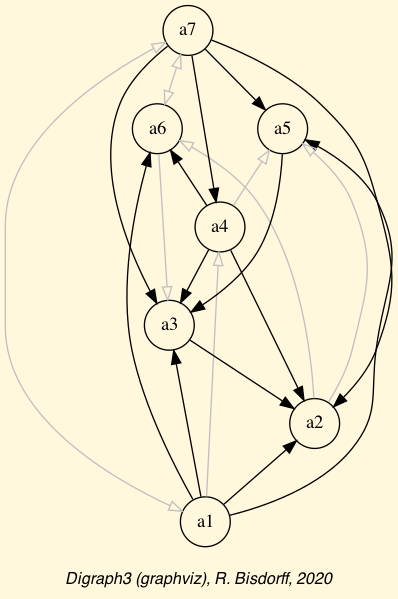
\includegraphics[width=5cm]{Figures/codualOdg.png}
\caption{The codual outranking digraph. It becomes readily clear now from the picture above that both alternatives \texttt{a1}  and \texttt{a7} are {\em not outranked\/} by any other alternatives. Hence, \texttt{a1}  and \texttt{a7} appear as \emph{weak} \Condorcet winners and may be recommended as potential \emph{best} decision alternatives in this illustrative preference modelling example.}
\label{fig:3.1}       % Give a unique label
\end{figure}
 
Many more tools for exploiting bipolar-valued outranking digraphs are available in the \Digraph resources \citep{BIS-2021}.
\vspace{1cm}

The next, and main Part of the book, presents decision methods and tools, like computing a best choice recommendation, a linear ranking or a rating with multiple incommensurable criteria. We also introduce the main performance tableau models we are going to use.  

%%%%%%%%%%%%%%%%%%%%%%%%%%%%%%%%%%%%
\phantomsection
\addcontentsline{toc}{section}{Notes}
\section*{Notes}

The seminal work on outranking digraphs goes back to the seventies and eighties of the twentieth century when Bernard Roy \index{Roy@\textsl{B. Roy}} joined the just starting University Paris-Dauphine and founded there the '\emph{Laboratoire d’Analyse et de Modélisation de Systèmes pour l’Aide à la Décision}' (LAMSADE). The LAMSADE became the major site in the development of the outranking approach to multiple criteria decision aid. \citep*{ROY-1993}.

The ongoing success of the original \emph{outranking} concept stems from the fact that it is rooted in a sound pragamatism. The multiple criteria performance tableau, necessarily associated with a given outranking digraph, is indeed convincingly objective and meaningful \citep{ROY-1991}. And, ideas from social choice theory gave initially the insight that a pairwise voting mechanism à la \Condorcet could provide an order-statistical tool for aggregating a set of preference points of view into what M. Barbut\index{Barbut@\textsl{M. Barbut}} called the \emph{central} \Condorcet point of view (\citet{CON-1784} and \citet{BAR-1980}); in fact the median of the multiple preference points of view, at minimal absolute \Kendall's\index{Kendall@\textsl{M.G. Kendall}} ordinal correlation distance from all individual points of view (see Chapter~\ref{sec:16}).

Considering thus each performance criterion as a subset of unanimous voters and balancing the votes in favour against considerable counter-performances in disfavour gave eventually rise to the concept of \emph{outranking situation}, a distinctive feature of the Multiple Criteria Decision Aid approach \citep{BIS-2015}.  A modern definition would be : An alternative $x$ is said to \emph{outrank} alternative $y$ when – a \emph{significant majority} of criteria confirm that alternative $x$ has to be considered as \emph{at least as well performing as} an alternative $y$ (the \emph{concordance} argument); and – no discordant criterion opens to significant doubt the validity of the previous confirmation by revealing a considerable counter-performance of alternative $x$ compared to $y$ (the \emph{discordance} argument).

If the concordance argument was always well recieved, the discordance argument however, very confused in the beginning \citep{ROY-1966}, could only be handled in an epistemically correct and logically sound way by using a bipolar-valued epistemic logic (see Definition~\ref{def:outranking}, \citet{BIS-2013}). The outranking situation had consequently to recieve an explicit negative definition: An alternative $x$ is said to \emph{do not outrank} an alternative $y$ when – a \emph{significant majority} of criteria confirm that alternative $x$ has to be considered as \emph{not at least as well performing as} alternative $y$; and – no discordant criterion opens to significant doubt the validity of the previous confirmation by revealing a considerable \emph{better} performance of alternative $x$ compared to $y$.

Furthermore, the initial conjunctive aggregation of the concordance and discordance arguments had to be replaced by a disjunctive epistemic fusion operation, polarising in a logically and epistemically sound way the concordance with the discordance argument. This way, outranking  digraphs gain two very useful properties from a measure theoretical perspective. They are \emph{weakly complete} ; incomparability situations are no longer attested by the absence of outranking relations, but instead by epistemic indeterminateness. And they verify the \emph{coduality principle}: the negation of the epistemic ``\emph{at least as well performing as}'' situation corresponds formally to the strict converse epistemic ``\emph{less well performing than}'' situation.


%%%%%%% The chapter bibliography
%\normallatexbib
\clearpage
%\phantomsection
% \addcontentsline{toc}{section}{Chapter Bibliography}
\bibliographystyle{spbasic}
%\typeout{}
\bibliography{03-backMatters/reference}
%\chapter{Working with outranking digraphs}
\label{sec:3}

\abstract*{ In this chapter, we introduce the main formal object of this book, namely the bipolar-valued outranking digraph. With a randomly generated multiple criteria performance tableau, we construct the corresponding bipolar-valued outranking relation from pairwise comparisons. The resulting bipolar-valued outranking characteristics may be recoded. Finally, the codual outranking digraph gives us the associated strict outranking relation.}

\begin{quotation}
``\emph{The rule for the combination of independent concurrent arguments takes a very simple form when expressed in terms of the intensity of belief ... It is this: Take the sum of all the feelings of belief which would be produced separately by all the arguments pro, subtract from that the similar sum for arguments con, and the remainder is the feeling of belief which ought to have the whole. This is a proceeding which men often resort to, under the name of balancing reasons.}'' -- C.S. Peirce, The probability of induction (1878)
\end{quotation}
\vspace{1cm}

\abstract{ In this chapter, we introduce the main formal object of this book, namely the bipolar-valued outranking digraph. With a randomly generated multiple criteria performance tableau, we construct the corresponding bipolar-valued outranking relation from pairwise comparisons. The resulting bipolar-valued outranking characteristics may be recoded. Finally, the codual outranking digraph gives us the associated strict outranking relation.}


\section{The hybrid outranking digraph model}
\label{sec:3.1}

In the \texttt{outrankingDigraphs} module\index{outrankingDigraphs@\texttt{outrankingDigraphs} module}, the \texttt{BipolarOutrankingDigraph}\index{BipolarOutrankingDigraph@\texttt{BipolarOutrankingDigraph} class} class provides our standard \emph{outranking digraph} constructor. Such an instance represents a \emph{hybrid} object of both the \texttt{PerformanceTableau} type \emph{and} the \texttt{Outran\-kingDigraph} type \citep{BIS-2021b}.

A given \texttt{BipolarOutrankingDigraph} object contains hence always at least the following attributes:
\begin{enumerate}[topsep=3pt,partopsep=0pt]
\item \texttt{actions}: an ordered dictionary describing the potential decision actions or alternatives with \texttt{name} and \texttt{comment} attributes,
\item \texttt{objectives}: a possibly empty ordered dictionary of decision objectives with \texttt{name} and \texttt{comment} attributes, describing the multiple preference dimensions involved in the decision problem, 
\item \texttt{criteria}: an ordered dictionary of performance criteria, i.e. \emph{preferentially independent} and \emph{non-redundant} decimal-valued evaluation functions used for assessng the performance of each potential decision action with respect to a decision objective,
\item \texttt{evaluation}: a double dictionary gathering performance evaluations for each decision alternative on each criterion function. 
\item \texttt{valuationdomain}: a dictionary with three entries: the minimum ($-1.0$, \emph{certainly outranked}), the median ($0.0$, \emph{indeterminate}) and the maximum characteristic value ($+1.0$, \emph{certainly outranking}),
\item \texttt{relation}: a double dictionary defined on the Cartesian product of the set of decision alternatives capturing the credibility of the pairwise \emph{outranking situation} computed on the basis of the performance differences observed between couples of decision alternatives on the given family of criteria functions.   
\end{enumerate}

Let us consider, for instance, a random bipolar-valued outranking digraph with seven decision actions denoted \texttt{a1}, \texttt{a2}, ..., \texttt{a7}. We need therefore, first, to generate in Listing~\vref{list:3.1} a corresponding random performance tableau.
\begin{lstlisting}[caption={Generating a random performance tableau.},label=list:3.1]
>>> from perfTabs import RandomPerformanceTableau
>>> pt = RandomPerformanceTableau(numberOfActions=7,\
...                               seed=100)   
>>> pt
   *------- PerformanceTableau instance description ------*
    Instance class     : RandomPerformanceTableau
    Seed               : 100
    Instance name      : randomperftab
    Actions            : 7
    Criteria           : 7
    NaN proportion (%) : 6.1
>>> pt.showActions()
  *----- show digraphs actions --------------*
   key:  a1
    name:       action 1
    comment:    RandomPerformanceTableau() generated.
   key:  a2
    name:       action 2
    comment:    RandomPerformanceTableau() generated.
     ...
     ...
   key:  a7
    name:       action 7
    comment:    RandomPerformanceTableau() generated.
\end{lstlisting}

In this example we consider a family of seven \emph{equisignificant} cardinal \emph{criteria functions} \texttt{g1}, \texttt{g2}, ..., \texttt{g7}, measuring the performance of each alternative on a rational scale from $0.0$ (worst) to $100.00$ (best). In order to capture the evaluation procedures' potential \emph{uncertainty} and \emph{imprecision}, each criterion function \texttt{g1} to \texttt{g7} admits three performance \emph{discrimination thresholds} of $2.5$, $5.0$ and $80.0$ pts for warranting respectively any \emph{indifference}, \emph{preference} or \emph{considerable performance difference} situation.
\begin{lstlisting}[caption={Inspecting the performance criteria.},label=list:3.2]
>>> pt.showCriteria()
  *----  criteria -----*
   g1 'RandomPerformanceTableau() instance'
     Scale = [0.0, 100.0]
     Weight = 1.0
     Threshold ind : 2.50 + 0.00x ; percentile: 4.76
     Threshold pref : 5.00 + 0.00x ; percentile: 9.52
     Threshold veto : 80.00 + 0.00x ; percentile: 95.24
   g2 'RandomPerformanceTableau() instance'
     Scale = [0.0, 100.0]
     Weight = 1.0
     Threshold ind : 2.50 + 0.00x ; percentile: 6.67
     Threshold pref : 5.00 + 0.00x ; percentile: 6.67
     Threshold veto : 80.00 + 0.00x ; percentile: 100.00
      ...
      ...
   g7 'RandomPerformanceTableau() instance'
     Scale = [0.0, 100.0]
     Weight = 1.0
     Threshold ind : 2.50 + 0.00x ; percentile: 0.00
     Threshold pref : 5.00 + 0.00x ; percentile: 4.76
     Threshold veto : 80.00 + 0.00x ; percentile: 100.00
\end{lstlisting}

On criteria function \texttt{g1} (see Lines 6-8 in List.~\vref{list:3.2}) we observe, for instance, about $5\%$ of \emph{indifference} situations, about $90\%$ of \emph{preference} situations and about $5\%$ of \emph{considerable} performance difference situations.

The individual \emph{performance evaluation} of all decision alternative on each criterion are gathered in a \emph{performance table}.\index{showPerformanceTableau@\texttt{showPerformanceTableau()}}
\begin{lstlisting}[caption={Inspecting the performance evaluations},label=list:3.3]
>>> pt.showPerformanceTableau()
    *----  performance tableau -----*
     criteria |  'a1'  'a2'  'a3'  'a4'  'a5'  'a6'  'a7'   
     ---------|------------------------------------------
      'g1'    |  15.2  44.5  57.9  58.0  24.2  29.1  96.6  
      'g2'    |  82.3  43.9   NA   35.8  29.1  34.8  62.2  
      'g3'    |  44.2  19.1  27.7  41.5  22.4  21.5  56.9  
      'g4'    |  46.4  16.2  21.5  51.2  77.0  39.4  32.1  
      'g5'    |  47.7  14.8  79.7  67.5   NA   90.7  80.2  
      'g6'    |  69.6  45.5  22.0  33.8  31.8   NA   48.8  
      'g7'    |  82.9  41.7  12.8  21.9  75.7  15.4   6.0  
\end{lstlisting}

It is noteworthy to mention the three \emph{missing data} (\texttt{NA}) cases: action \texttt{a3} is missing, for instance, an evaluation on criterion \texttt{g2} (see Line 6 in List.~\vref{list:3.3}).
    
\section{The bipolar-valued outranking digraph}
\label{sec:3.2}

Given the previous random performance tableau \texttt{pt}, the \texttt{BipolarOutranking\-Digraph}\index{BipolarOutrankingDigraph@\texttt{BipolarOutrankingDigraph}} class constructor computes the corresponding \emph{bipolar-valued outranking digraph}. 
\begin{lstlisting}[caption={Example of random bipolar-valued outranking digraph.},label=list:3.4]
>>> from outrankingDigraphs import \
...                       BipolarOutrankingDigraph
>>> odg = BipolarOutrankingDigraph(pt)
>>> odg
  *------- Object instance description ------*
   Instance class       : BipolarOutrankingDigraph
   Instance name        : rel_randomperftab
   Actions              : 7
   Criteria             : 7
   Size                 : 20
   Determinateness (%)  : 63.27
   Valuation domain     : [-1.00;1.00]
   Attributes           : [
        'name', 'actions', 
	'criteria', 'evaluation', 'NA',
	'valuationdomain', 'relation', 
	'order', 'gamma', 'notGamma', ...
	]
\end{lstlisting}

The resulting digraph contains 20 positive (valid) outranking relations. And, the mean majority criteria significance support of all the pairwise outranking situations is $63.3\%$ (see Lines 9-10 in List.~\vref{list:3.4}).

We may inspect the complete $[-1.0,+1.0]$-valued adjacency table with the \texttt{showRelationTable()} method().\index{showRelationTable@\texttt{showRelationTable()}}
\begin{lstlisting}[caption={Inspecting the valued adjacency table.},label=list:3.5]
>>> odg.showRelationTable()
  * ---- Relation Table -----
   r(x,y)|  'a1'   'a2'   'a3'   'a4'   'a5'   'a6'   'a7'   
   ------|-------------------------------------------------
    'a1' | +1.00  +0.71  +0.29  +0.29  +0.29  +0.29  +0.00  
    'a2' | -0.71  +1.00  -0.29  -0.14  +0.14  +0.29  -0.57  
    'a3' | -0.29  +0.29  +1.00  -0.29  -0.14  +0.00  -0.29  
    'a4' | +0.00  +0.14  +0.57  +1.00  +0.29  +0.57  -0.43  
    'a5' | -0.29  +0.00  +0.14  +0.00  +1.00  +0.29  -0.29  
    'a6' | -0.29  +0.00  +0.14  -0.29  +0.14  +1.00  +0.00  
    'a7' | +0.00  +0.71  +0.57  +0.43  +0.29  +0.00  +1.00  
   Valuation domain: [-1.0; 1.0]
\end{lstlisting}

The \texttt{BipolarOutrankingDigraph}\index{BipolarOutrankingDigraph@\texttt{BipolarOutrankingDigraph}} class constructor computes from the given performance tableau $pt$ the characteristic value $r(x \succsim y)$ of a \emph{pairwise outranking} relation $x\, \succsim \,y$ in a default \emph{valuation domain} $[-1.0,+1.0]$ with the {\em median\/} value $0.0$ acting as \emph{indeterminate} characteristic value\footnote{See Definition~\vref{def:3.1} \citep{BIS-2013}}. 

\begin{definition}[Semantics of the bipolar-valued characteristic function $r$]\label{def:3.1}

\noindent The semantics of $r(x \succsim y)$ are the following:
\begin{itemize}[nosep]
\item [a.] When $r(x \succsim y) > 0.0$, it is more {\em True\/} than {\em False\/} that $x$ \emph{outranks} $y$, i.e. alternative $x$ is ``\emph{at least as well evaluated as}'' alternative $y$ on a weighted majority of criteria {\bf and} there is no considerable negative performance difference observed in disfavour of $x$,
\item [b.] When $r(x \succsim y) < 0.0$, it is more {\em False\/} than {\em True\/} that $x$ \emph{outranks} $y$, i.e. alternative $x$ is {\bf not} ``\emph{at least as well evaluated as} alternative $y$ on a weighted majority of criteria than alternative $y$ {\bf and} there is no considerable positive performance difference observed in favour of $x$,
\item [c.] When $r(x \succsim y) = 0.0$, it is {\bf indeterminate} whether $x$ outranks $y$ or not.
\end{itemize}
\end{definition}

\section{Pairwise comparisons}
\label{sec:3.3}

From above given semantics, we notice in line 5 in Listing~\vref{list:3.5} that \texttt{a1} outranks \texttt{a2}: $r(a1 \succsim a2) + 0.71$), but not \texttt{a7}: $r(a1 \succsim a7) = 0.0$). In order to comprehend the characteristic values shown in the outranking relation table, we can inspect with the \texttt{showPairwiseComparison()} method\index{showPairwiseComparison@\texttt{showPairwiseComparison()}} the details of the pairwise multiple criteria comparison between, for instance, alternatives \texttt{a1} and \texttt{a2}.
\begin{lstlisting}[caption={Inspecting a pairwise multiple criteria comparison},label=list:3.6]
>>> odg.showPairwiseComparison('a1','a2')
  *------------  pairwise comparison ----*
   Comparing actions : (a1, a2)
   crit. wght. g(a1)  g(a2)   diff  | ind   pref    r() 
   -------------------------------  	 --------------------
    g1   1.00  15.17  44.51  -29.34 | 2.50  5.00   -1.00 
    g2   1.00  82.29  43.90  +38.39 | 2.50  5.00   +1.00 
    g3   1.00  44.23  19.10  +25.13 | 2.50  5.00   +1.00 
    g4   1.00  46.37  16.22  +30.15 | 2.50  5.00   +1.00 
    g5   1.00  47.67  14.81  +32.86 | 2.50  5.00   +1.00 
    g6   1.00  69.62  45.49  +24.13 | 2.50  5.00   +1.00 
    g7   1.00  82.88  41.66  +41.22 | 2.50  5.00   +1.00 
    Valuation in range: -7.00 to +7.00;          -------
       r(a1,a2): +5.00/7.00 = +0.71                +5.00
\end{lstlisting}

The outranking characteristic value $r(a1 \succsim a2)$ represents the relative \emph{majority margin} resulting from the difference between the significance weights of the criteria in favour and the significance weights of the criteria in disfavour of the statement that alternative \texttt{a1} is ``\emph{at least as well evaluated as}'' alternative \texttt{a2}. No considerable performance difference being observed, no polarising situation is triggered in this pairwise comparison.

Such a polarised situation is however observed when we compare the evaluations of alternatives \texttt{a1} and \texttt{a7} with the \texttt{showPairwiseOutrankings()} method. \index{showPairwiseoutrankings@\texttt{showPairwiseOutrankings()}}
\begin{lstlisting}[caption={Pairwise comparison with considerable performance difference},label=list:3.7,basicstyle=\ttfamily\scriptsize]
>>> odg.showPairwiseoutrankings('a1','a7')
  *------------  pairwise comparison ----*
   Comparing actions : (a1, a7)
   crit. wght. g(a1)  g(a7)   diff  | ind   pref    r()  |  v     veto
   -------------------------------   ------------------   -----------
    g1   1.00  15.17  96.58  -81.41 | 2.50  5.00   -1.00 | 80.00 -1.00
    g2   1.00  82.29  62.22  +20.07 | 2.50  5.00   +1.00 | 
    g3   1.00  44.23  56.90  -12.67 | 2.50  5.00   -1.00 | 
    g4   1.00  46.37  32.06  +14.31 | 2.50  5.00   +1.00 | 
    g5   1.00  47.67  80.16  -32.49 | 2.50  5.00   -1.00 | 
    g6   1.00  69.62  48.80  +20.82 | 2.50  5.00   +1.00 | 
    g7   1.00  82.88   6.05  +76.83 | 2.50  5.00   +1.00 | 
   ----------------------------------------
   Valuation in range: -7.00 to +7.00; r(x,y)= +1/7 => 0.0
  *------------  pairwise comparison ----*
   Comparing actions : (a1, a7)
   crit. wght. g(a7)  g(a1)   diff  | ind   pref    r()  |  v     veto
   -------------------------------   ------------------   -----------
    g1   1.00  96.58  15.17  +81.41 | 2.50  5.00   +1.00 | 80.00 +1.00
    g2   1.00  62.22  82.29  -20.07 | 2.50  5.00   -1.00 | 
    g3   1.00  56.90  44.23  +12.67 | 2.50  5.00   +1.00 | 
    g4   1.00  32.06  46.37  -14.31 | 2.50  5.00   -1.00 | 
    g5   1.00  80.16  47.67  +32.49 | 2.50  5.00   +1.00 | 
    g6   1.00  48.80  69.62  -20.82 | 2.50  5.00   -1.00 | 
    g7   1.00   6.05  82.88  -76.83 | 2.50  5.00   -1.00 | 
   ----------------------------------------
   Valuation in range: -7.00 to +7.00; r(x,y)= -1/7 => 0.0
\end{lstlisting}

This time, we observe a $(1/7 + 1)/2 = 57.1\%$ majority of criteria significance warranting a ``\emph{at least as well evaluated as}'' situation between alternative \texttt{a1} and alternative \texttt{a7}. Yet, we also observe a considerable \emph{negative} performance difference on criterion \texttt{g1} (see Line 6 in List.~\vref{list:3.7}). Both contradictory facts trigger eventually in Line 14 an \emph{indeterminate} outranking situation. The inverse polarisation effect appears when considering in Lines 19-25 the converse performance differences between alternative \texttt{a7} and alternative \texttt{a1}. The considerable better performing situation on criterion \texttt{g1} makes doubtful the otherwise ``\emph{not at least as well evaluated as}'' situation (see Lines 19 and 27).

Notice that the occurrence in a pairwise comparison of conjointly considerable positive and negative performance differences will also trigger an indeterminate outranking situation. When observing at the same time a positive (resp. negative) ``\emph{at least as well evaluated as}'' situation and one or more considerable positive (resp. negative) performance difference, the outranking situation gets validated (resp. invalidated) for certain \citep{BIS-2013}.

\section{Recoding the characteristic valuation domain}
\label{sec:3.4}

All outranking digraphs, being of root \texttt{Digraph} type, inherit the methods available under this latter class. The characteristic valuation domain of a digraph can, for instance, be recoded with the \texttt{recodeValuation()}\index{recodeValuation@\emph{recodeValuation()}} method to the \emph{integer} range $[-7,+7]$, i.e. plus or minus the total significance weights of the family of criteria considered in this example instance \texttt{odg}.
\begin{lstlisting}[caption={Recoding the digraph valuation},label=list:3.8]
>>> odg.recodeValuation(-7,+7)
>>> odg.valuationdomain['hasIntegerValuation'] = True
>>> Digraph.showRelationTable(odg,ReflexiveTerms=False)
  * ---- Relation Table -----
   r(x,y)  |  'a1'  'a2'  'a3'  'a4'  'a5'  'a6'  'a7'	  
  ---------|------------------------------------------
    'a1'   |    -    +5    +2    +2    +2    +2     0	 
    'a2'   |   -5     -    -1    -1    +1    +2    -4	 
    'a3'   |   -1    +2     -    -1    -1     0    -1	 
    'a4'   |    0    +1    +4     -    +2    +4    -3	 
    'a5'   |   -1     0    +1     0     -    +2    -1	 
    'a6'   |   -1     0    +1    -1    +1     -     0	 
    'a7'   |    0    +5    +4    +3    +2     0     -	 
    Valuation domain: [-7;+7]
\end{lstlisting}

Notice in Listing~\vref{list:3.8} that the self comparison characteristics $r(x \succsim x)$ may be ignored by setting the \texttt{ReflexiveTerms} Boolean parameter to \texttt{False}. Mind that the trivial reflexive terms of outranking relations are ignored in some of the \Digraph methods. 

\section{The strict outranking digraph}
\label{sec:3.5}

From theory we know that a bipolar-valued outranking digraph is \emph{weakly complete}, i.e. if $r(x \succsim y) < 0.0$ then $r(y \succsim x) \geq 0.0$. From this property follows that a bipolar-valued outranking digraph verifies the \emph{coduality principle}\index{coduality principle}: the \emph{dual}\footnote{Not to be confused with the dual graph of a plane graph $g$ that has a vertex for each face of $g$. Here we mean the \emph{less than} (strict converse) relation corresponding to a \emph{greater or equal} relation, or the \emph{less than or equal} relation corresponding to a (strict) \emph{better than} relation.} --strict negation-- of the \emph{converse} --inverse-- of the outranking relation $(x \succsim y)$ corresponds to its asymmetric \emph{strict outranking} part $(x \succnsim y)$  \citep{BIS-2013, ADT-L7}.

We may visualize the \emph{codual} (\emph{strict}) outranking digraph with a graphviz drawing \footnote{The \texttt{exportGraphViz()} method is depending on drawing tools from the graphviz software (https://graphviz.org/). On Linux Ubuntu or Debian you may try \texttt{sudo apt-get install graphviz} to install them. There are ready \emph{dmg} installers for Mac OSX.}.\index{graphviz}
\begin{lstlisting}
>>> cdodg = -(~odg)
>>> cdodg.exportGraphViz('codualOdg')
  *---- exporting a dot file for GraphViz tools ---------*
   Exporting to codualOdg.dot
   dot -Grankdir=BT -Tpng codualOdg.dot -o codualOdg.png
\end{lstlisting}
\begin{figure}[ht]
\sidecaption[t]
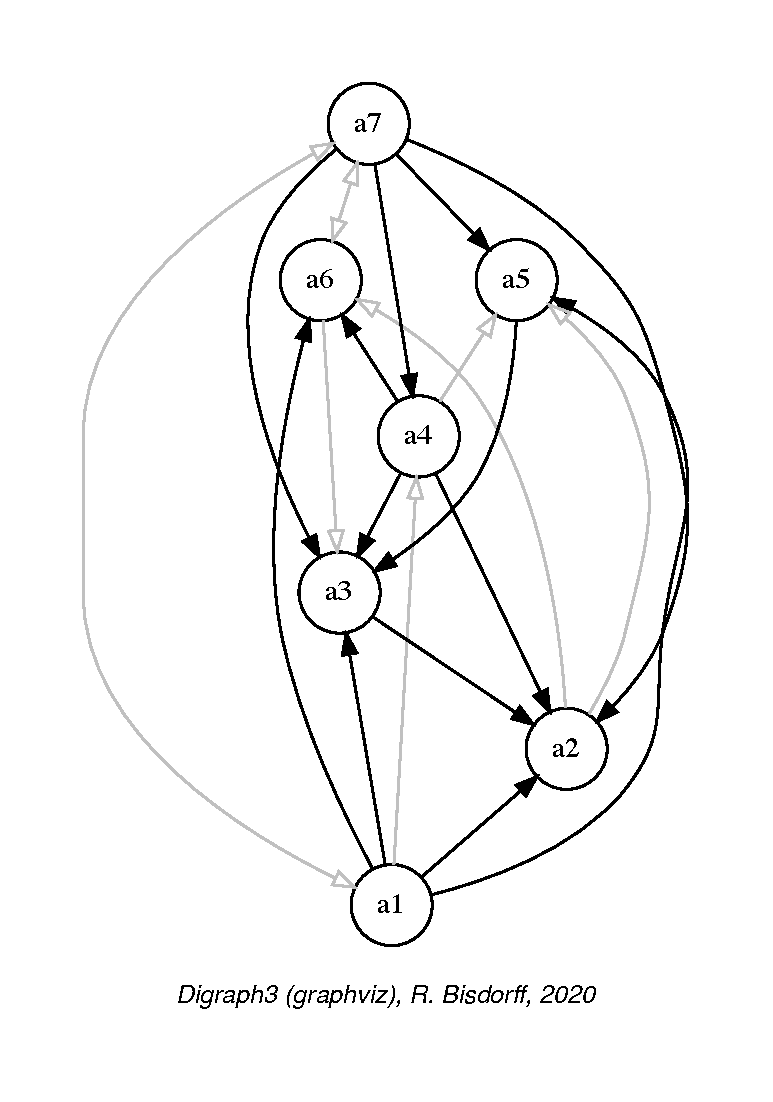
\includegraphics[width=5cm]{Figures/3-1-codualOdg.pdf}
\caption[The strict (codual) outranking digraph]{The strict (codual) outranking digraph. It becomes readily clear now from the picture that both alternatives \texttt{a1}  and \texttt{a7} are \emph{not outranked} by any other alternatives. Hence, \texttt{a1}  and \texttt{a7} appear as \emph{weak} \Condorcet winners and may be recommended as potential \emph{best} decision alternatives in this illustrative preference modelling example}
\label{fig:3.1}       % Give a unique label
\end{figure}
 
Many more tools for exploiting bipolar-valued outranking digraphs are available in the \Digraph resources \citep{BIS-2021b}.
\vspace{1cm}

In the methodological Part II, we present and discuss multiple criteria evaluation models and decision algorithms, like building a best choice recommendation, determining the winner of an election, computing linear rankings or quantile ratings with multiple incommensurable criteria.

%%%%%%%%%%%%%%%%%%%%%%%%%%%%%%%%%%%%
\phantomsection
\addcontentsline{toc}{section}{Notes}
\section*{Notes}

The seminal work on outranking digraphs goes back to the seventies and eighties when Bernard Roy \index{Roy@\textsl{B. Roy}} joined the just starting University Paris-Dauphine and founded there the '\emph{Laboratoire d’Analyse et de Modélisation de Systèmes pour l’Aide à la Décision}' (LAMSADE). The LAMSADE became the major site in the development of the outranking approach to multiple criteria decision aid. \citep*{ROY-1993}.

The ongoing success of the original \emph{outranking} concept stems from the fact that it is rooted in a sound pragmatism. The multiple criteria performance tableau, necessarily associated with a given outranking digraph, is indeed convincingly objective and meaningful \citep{ROY-1991}. And, ideas from social choice theory gave initially the insight that a pairwise voting mechanism à la \Condorcet could provide an order-statistical tool for aggregating a set of preference points of view into what M. Barbut\index{Barbut@\emph{M. Barbut}} called the \emph{central} \Condorcet point of view (\citealp{CON-1784} and \citealp{BAR-1980}); in fact the median of the multiple preference points of view, at minimal absolute \Kendall's\index{Kendall@\emph{M.G. Kendall}} ordinal correlation distance from all individual points of view (see Chap.~\ref{sec:16}).

Considering thus each performance criterion as a subset of unanimous voters and balancing the votes in favour against considerable counter-performances in disfavour gave eventually rise to the concept of \emph{outranking situation}, a distinctive feature of the Multiple Criteria Decision Aid approach \citep{BIS-2015}.  A modern definition would be : An alternative $x$ is said to \emph{outrank} alternative $y$ when – a \emph{significant majority} of criteria confirm that alternative $x$ has to be considered as \emph{at least as well evaluated as} an alternative $y$ (the \emph{concordance} argument); and – no discordant criterion opens to significant doubt the validity of the previous confirmation by revealing a considerable counter-performance of alternative $x$ compared to $y$ (the \emph{discordance} argument).

If the concordance argument was always well received, the discordance argument however, very confused in the beginning \citep{ROY-1966}, could only be handled in an epistemically correct and logically sound way by using a bipolar-valued epistemic logic (see Def.~\vref{def:3.1} and \citealp{BIS-2013}). The outranking situation had consequently to receive an explicit negative definition: An alternative $x$ is said to \emph{do not outrank} an alternative $y$ when – a \emph{significant majority} of criteria confirm that alternative $x$ has to be considered as \emph{not at least as well evaluated as} alternative $y$; and – no discordant criterion opens to significant doubt the validity of the previous confirmation by revealing a considerable \emph{better} performance of alternative $x$ compared to $y$.

Furthermore, the initial conjunctive aggregation of the concordance and discordance arguments had to be replaced by a disjunctive epistemic fusion operation, polarising in a logically and epistemically sound way the concordance with the discordance argument. This way, bipolar-valued outranking  digraphs gain two very useful properties from a measure theoretical perspective. They are \emph{weakly complete}; incomparability situations are no longer attested by the absence of positive outranking relations, but instead by epistemic indeterminateness. And they verify the \emph{coduality principle}: the negation of the epistemic ``\emph{at least as well evaluated as}'' situation corresponds formally to the strict converse epistemic ``\emph{less well evaluated than}'' situation.


%%%%%%% The chapter bibliography
%\normallatexbib
\clearpage
%\phantomsection
%\addcontentsline{toc}{section}{Chapter Bibliography}
%\chapter{Working with outranking digraphs}
\label{sec:3}

\abstract*{ In this chapter, we introduce the main formal object of this book, namely the bipolar-valued outranking digraph. With a randomly generated multiple criteria performance tableau, we construct the corresponding bipolar-valued outranking relation from pairwise comparisons. The resulting bipolar-valued outranking characteristics may be recoded. Finally, the codual outranking digraph gives us the associated strict outranking relation.}

\begin{quotation}
``\emph{The rule for the combination of independent concurrent arguments takes a very simple form when expressed in terms of the intensity of belief ... It is this: Take the sum of all the feelings of belief which would be produced separately by all the arguments pro, subtract from that the similar sum for arguments con, and the remainder is the feeling of belief which ought to have the whole. This is a proceeding which men often resort to, under the name of balancing reasons.}'' -- C.S. Peirce, The probability of induction (1878)
\end{quotation}
\vspace{1cm}

\abstract{ In this chapter, we introduce the main formal object of this book, namely the bipolar-valued outranking digraph. With a randomly generated multiple criteria performance tableau, we construct the corresponding bipolar-valued outranking relation from pairwise comparisons. The resulting bipolar-valued outranking characteristics may be recoded. Finally, the codual outranking digraph gives us the associated strict outranking relation.}


\section{The hybrid outranking digraph model}
\label{sec:3.1}

In the \texttt{outrankingDigraphs} module\index{outrankingDigraphs@\texttt{outrankingDigraphs} module}, the \texttt{BipolarOutrankingDigraph}\index{BipolarOutrankingDigraph@\texttt{BipolarOutrankingDigraph} class} class provides our standard \emph{outranking digraph} constructor. Such an instance represents a \emph{hybrid} object of both the \texttt{PerformanceTableau} type \emph{and} the \texttt{Outran\-kingDigraph} type \citep{BIS-2021b}.

A given \texttt{BipolarOutrankingDigraph} object contains hence always at least the following attributes:
\begin{enumerate}[topsep=3pt,partopsep=0pt]
\item \texttt{actions}: an ordered dictionary describing the potential decision actions or alternatives with \texttt{name} and \texttt{comment} attributes,
\item \texttt{objectives}: a possibly empty ordered dictionary of decision objectives with \texttt{name} and \texttt{comment} attributes, describing the multiple preference dimensions involved in the decision problem, 
\item \texttt{criteria}: an ordered dictionary of performance criteria, i.e. \emph{preferentially independent} and \emph{non-redundant} decimal-valued evaluation functions used for assessng the performance of each potential decision action with respect to a decision objective,
\item \texttt{evaluation}: a double dictionary gathering performance evaluations for each decision alternative on each criterion function. 
\item \texttt{valuationdomain}: a dictionary with three entries: the minimum ($-1.0$, \emph{certainly outranked}), the median ($0.0$, \emph{indeterminate}) and the maximum characteristic value ($+1.0$, \emph{certainly outranking}),
\item \texttt{relation}: a double dictionary defined on the Cartesian product of the set of decision alternatives capturing the credibility of the pairwise \emph{outranking situation} computed on the basis of the performance differences observed between couples of decision alternatives on the given family of criteria functions.   
\end{enumerate}

Let us consider, for instance, a random bipolar-valued outranking digraph with seven decision actions denoted \texttt{a1}, \texttt{a2}, ..., \texttt{a7}. We need therefore, first, to generate in Listing~\vref{list:3.1} a corresponding random performance tableau.
\begin{lstlisting}[caption={Generating a random performance tableau.},label=list:3.1]
>>> from perfTabs import RandomPerformanceTableau
>>> pt = RandomPerformanceTableau(numberOfActions=7,\
...                               seed=100)   
>>> pt
   *------- PerformanceTableau instance description ------*
    Instance class     : RandomPerformanceTableau
    Seed               : 100
    Instance name      : randomperftab
    Actions            : 7
    Criteria           : 7
    NaN proportion (%) : 6.1
>>> pt.showActions()
  *----- show digraphs actions --------------*
   key:  a1
    name:       action 1
    comment:    RandomPerformanceTableau() generated.
   key:  a2
    name:       action 2
    comment:    RandomPerformanceTableau() generated.
     ...
     ...
   key:  a7
    name:       action 7
    comment:    RandomPerformanceTableau() generated.
\end{lstlisting}

In this example we consider a family of seven \emph{equisignificant} cardinal \emph{criteria functions} \texttt{g1}, \texttt{g2}, ..., \texttt{g7}, measuring the performance of each alternative on a rational scale from $0.0$ (worst) to $100.00$ (best). In order to capture the evaluation procedures' potential \emph{uncertainty} and \emph{imprecision}, each criterion function \texttt{g1} to \texttt{g7} admits three performance \emph{discrimination thresholds} of $2.5$, $5.0$ and $80.0$ pts for warranting respectively any \emph{indifference}, \emph{preference} or \emph{considerable performance difference} situation.
\begin{lstlisting}[caption={Inspecting the performance criteria.},label=list:3.2]
>>> pt.showCriteria()
  *----  criteria -----*
   g1 'RandomPerformanceTableau() instance'
     Scale = [0.0, 100.0]
     Weight = 1.0
     Threshold ind : 2.50 + 0.00x ; percentile: 4.76
     Threshold pref : 5.00 + 0.00x ; percentile: 9.52
     Threshold veto : 80.00 + 0.00x ; percentile: 95.24
   g2 'RandomPerformanceTableau() instance'
     Scale = [0.0, 100.0]
     Weight = 1.0
     Threshold ind : 2.50 + 0.00x ; percentile: 6.67
     Threshold pref : 5.00 + 0.00x ; percentile: 6.67
     Threshold veto : 80.00 + 0.00x ; percentile: 100.00
      ...
      ...
   g7 'RandomPerformanceTableau() instance'
     Scale = [0.0, 100.0]
     Weight = 1.0
     Threshold ind : 2.50 + 0.00x ; percentile: 0.00
     Threshold pref : 5.00 + 0.00x ; percentile: 4.76
     Threshold veto : 80.00 + 0.00x ; percentile: 100.00
\end{lstlisting}

On criteria function \texttt{g1} (see Lines 6-8 in List.~\vref{list:3.2}) we observe, for instance, about $5\%$ of \emph{indifference} situations, about $90\%$ of \emph{preference} situations and about $5\%$ of \emph{considerable} performance difference situations.

The individual \emph{performance evaluation} of all decision alternative on each criterion are gathered in a \emph{performance table}.\index{showPerformanceTableau@\texttt{showPerformanceTableau()}}
\begin{lstlisting}[caption={Inspecting the performance evaluations},label=list:3.3]
>>> pt.showPerformanceTableau()
    *----  performance tableau -----*
     criteria |  'a1'  'a2'  'a3'  'a4'  'a5'  'a6'  'a7'   
     ---------|------------------------------------------
      'g1'    |  15.2  44.5  57.9  58.0  24.2  29.1  96.6  
      'g2'    |  82.3  43.9   NA   35.8  29.1  34.8  62.2  
      'g3'    |  44.2  19.1  27.7  41.5  22.4  21.5  56.9  
      'g4'    |  46.4  16.2  21.5  51.2  77.0  39.4  32.1  
      'g5'    |  47.7  14.8  79.7  67.5   NA   90.7  80.2  
      'g6'    |  69.6  45.5  22.0  33.8  31.8   NA   48.8  
      'g7'    |  82.9  41.7  12.8  21.9  75.7  15.4   6.0  
\end{lstlisting}

It is noteworthy to mention the three \emph{missing data} (\texttt{NA}) cases: action \texttt{a3} is missing, for instance, an evaluation on criterion \texttt{g2} (see Line 6 in List.~\vref{list:3.3}).
    
\section{The bipolar-valued outranking digraph}
\label{sec:3.2}

Given the previous random performance tableau \texttt{pt}, the \texttt{BipolarOutranking\-Digraph}\index{BipolarOutrankingDigraph@\texttt{BipolarOutrankingDigraph}} class constructor computes the corresponding \emph{bipolar-valued outranking digraph}. 
\begin{lstlisting}[caption={Example of random bipolar-valued outranking digraph.},label=list:3.4]
>>> from outrankingDigraphs import \
...                       BipolarOutrankingDigraph
>>> odg = BipolarOutrankingDigraph(pt)
>>> odg
  *------- Object instance description ------*
   Instance class       : BipolarOutrankingDigraph
   Instance name        : rel_randomperftab
   Actions              : 7
   Criteria             : 7
   Size                 : 20
   Determinateness (%)  : 63.27
   Valuation domain     : [-1.00;1.00]
   Attributes           : [
        'name', 'actions', 
	'criteria', 'evaluation', 'NA',
	'valuationdomain', 'relation', 
	'order', 'gamma', 'notGamma', ...
	]
\end{lstlisting}

The resulting digraph contains 20 positive (valid) outranking relations. And, the mean majority criteria significance support of all the pairwise outranking situations is $63.3\%$ (see Lines 9-10 in List.~\vref{list:3.4}).

We may inspect the complete $[-1.0,+1.0]$-valued adjacency table with the \texttt{showRelationTable()} method().\index{showRelationTable@\texttt{showRelationTable()}}
\begin{lstlisting}[caption={Inspecting the valued adjacency table.},label=list:3.5]
>>> odg.showRelationTable()
  * ---- Relation Table -----
   r(x,y)|  'a1'   'a2'   'a3'   'a4'   'a5'   'a6'   'a7'   
   ------|-------------------------------------------------
    'a1' | +1.00  +0.71  +0.29  +0.29  +0.29  +0.29  +0.00  
    'a2' | -0.71  +1.00  -0.29  -0.14  +0.14  +0.29  -0.57  
    'a3' | -0.29  +0.29  +1.00  -0.29  -0.14  +0.00  -0.29  
    'a4' | +0.00  +0.14  +0.57  +1.00  +0.29  +0.57  -0.43  
    'a5' | -0.29  +0.00  +0.14  +0.00  +1.00  +0.29  -0.29  
    'a6' | -0.29  +0.00  +0.14  -0.29  +0.14  +1.00  +0.00  
    'a7' | +0.00  +0.71  +0.57  +0.43  +0.29  +0.00  +1.00  
   Valuation domain: [-1.0; 1.0]
\end{lstlisting}

The \texttt{BipolarOutrankingDigraph}\index{BipolarOutrankingDigraph@\texttt{BipolarOutrankingDigraph}} class constructor computes from the given performance tableau $pt$ the characteristic value $r(x \succsim y)$ of a \emph{pairwise outranking} relation $x\, \succsim \,y$ in a default \emph{valuation domain} $[-1.0,+1.0]$ with the {\em median\/} value $0.0$ acting as \emph{indeterminate} characteristic value\footnote{See Definition~\vref{def:3.1} \citep{BIS-2013}}. 

\begin{definition}[Semantics of the bipolar-valued characteristic function $r$]\label{def:3.1}

\noindent The semantics of $r(x \succsim y)$ are the following:
\begin{itemize}[nosep]
\item [a.] When $r(x \succsim y) > 0.0$, it is more {\em True\/} than {\em False\/} that $x$ \emph{outranks} $y$, i.e. alternative $x$ is ``\emph{at least as well evaluated as}'' alternative $y$ on a weighted majority of criteria {\bf and} there is no considerable negative performance difference observed in disfavour of $x$,
\item [b.] When $r(x \succsim y) < 0.0$, it is more {\em False\/} than {\em True\/} that $x$ \emph{outranks} $y$, i.e. alternative $x$ is {\bf not} ``\emph{at least as well evaluated as} alternative $y$ on a weighted majority of criteria than alternative $y$ {\bf and} there is no considerable positive performance difference observed in favour of $x$,
\item [c.] When $r(x \succsim y) = 0.0$, it is {\bf indeterminate} whether $x$ outranks $y$ or not.
\end{itemize}
\end{definition}

\section{Pairwise comparisons}
\label{sec:3.3}

From above given semantics, we notice in line 5 in Listing~\vref{list:3.5} that \texttt{a1} outranks \texttt{a2}: $r(a1 \succsim a2) + 0.71$), but not \texttt{a7}: $r(a1 \succsim a7) = 0.0$). In order to comprehend the characteristic values shown in the outranking relation table, we can inspect with the \texttt{showPairwiseComparison()} method\index{showPairwiseComparison@\texttt{showPairwiseComparison()}} the details of the pairwise multiple criteria comparison between, for instance, alternatives \texttt{a1} and \texttt{a2}.
\begin{lstlisting}[caption={Inspecting a pairwise multiple criteria comparison},label=list:3.6]
>>> odg.showPairwiseComparison('a1','a2')
  *------------  pairwise comparison ----*
   Comparing actions : (a1, a2)
   crit. wght. g(a1)  g(a2)   diff  | ind   pref    r() 
   -------------------------------  	 --------------------
    g1   1.00  15.17  44.51  -29.34 | 2.50  5.00   -1.00 
    g2   1.00  82.29  43.90  +38.39 | 2.50  5.00   +1.00 
    g3   1.00  44.23  19.10  +25.13 | 2.50  5.00   +1.00 
    g4   1.00  46.37  16.22  +30.15 | 2.50  5.00   +1.00 
    g5   1.00  47.67  14.81  +32.86 | 2.50  5.00   +1.00 
    g6   1.00  69.62  45.49  +24.13 | 2.50  5.00   +1.00 
    g7   1.00  82.88  41.66  +41.22 | 2.50  5.00   +1.00 
    Valuation in range: -7.00 to +7.00;          -------
       r(a1,a2): +5.00/7.00 = +0.71                +5.00
\end{lstlisting}

The outranking characteristic value $r(a1 \succsim a2)$ represents the relative \emph{majority margin} resulting from the difference between the significance weights of the criteria in favour and the significance weights of the criteria in disfavour of the statement that alternative \texttt{a1} is ``\emph{at least as well evaluated as}'' alternative \texttt{a2}. No considerable performance difference being observed, no polarising situation is triggered in this pairwise comparison.

Such a polarised situation is however observed when we compare the evaluations of alternatives \texttt{a1} and \texttt{a7} with the \texttt{showPairwiseOutrankings()} method. \index{showPairwiseoutrankings@\texttt{showPairwiseOutrankings()}}
\begin{lstlisting}[caption={Pairwise comparison with considerable performance difference},label=list:3.7,basicstyle=\ttfamily\scriptsize]
>>> odg.showPairwiseoutrankings('a1','a7')
  *------------  pairwise comparison ----*
   Comparing actions : (a1, a7)
   crit. wght. g(a1)  g(a7)   diff  | ind   pref    r()  |  v     veto
   -------------------------------   ------------------   -----------
    g1   1.00  15.17  96.58  -81.41 | 2.50  5.00   -1.00 | 80.00 -1.00
    g2   1.00  82.29  62.22  +20.07 | 2.50  5.00   +1.00 | 
    g3   1.00  44.23  56.90  -12.67 | 2.50  5.00   -1.00 | 
    g4   1.00  46.37  32.06  +14.31 | 2.50  5.00   +1.00 | 
    g5   1.00  47.67  80.16  -32.49 | 2.50  5.00   -1.00 | 
    g6   1.00  69.62  48.80  +20.82 | 2.50  5.00   +1.00 | 
    g7   1.00  82.88   6.05  +76.83 | 2.50  5.00   +1.00 | 
   ----------------------------------------
   Valuation in range: -7.00 to +7.00; r(x,y)= +1/7 => 0.0
  *------------  pairwise comparison ----*
   Comparing actions : (a1, a7)
   crit. wght. g(a7)  g(a1)   diff  | ind   pref    r()  |  v     veto
   -------------------------------   ------------------   -----------
    g1   1.00  96.58  15.17  +81.41 | 2.50  5.00   +1.00 | 80.00 +1.00
    g2   1.00  62.22  82.29  -20.07 | 2.50  5.00   -1.00 | 
    g3   1.00  56.90  44.23  +12.67 | 2.50  5.00   +1.00 | 
    g4   1.00  32.06  46.37  -14.31 | 2.50  5.00   -1.00 | 
    g5   1.00  80.16  47.67  +32.49 | 2.50  5.00   +1.00 | 
    g6   1.00  48.80  69.62  -20.82 | 2.50  5.00   -1.00 | 
    g7   1.00   6.05  82.88  -76.83 | 2.50  5.00   -1.00 | 
   ----------------------------------------
   Valuation in range: -7.00 to +7.00; r(x,y)= -1/7 => 0.0
\end{lstlisting}

This time, we observe a $(1/7 + 1)/2 = 57.1\%$ majority of criteria significance warranting a ``\emph{at least as well evaluated as}'' situation between alternative \texttt{a1} and alternative \texttt{a7}. Yet, we also observe a considerable \emph{negative} performance difference on criterion \texttt{g1} (see Line 6 in List.~\vref{list:3.7}). Both contradictory facts trigger eventually in Line 14 an \emph{indeterminate} outranking situation. The inverse polarisation effect appears when considering in Lines 19-25 the converse performance differences between alternative \texttt{a7} and alternative \texttt{a1}. The considerable better performing situation on criterion \texttt{g1} makes doubtful the otherwise ``\emph{not at least as well evaluated as}'' situation (see Lines 19 and 27).

Notice that the occurrence in a pairwise comparison of conjointly considerable positive and negative performance differences will also trigger an indeterminate outranking situation. When observing at the same time a positive (resp. negative) ``\emph{at least as well evaluated as}'' situation and one or more considerable positive (resp. negative) performance difference, the outranking situation gets validated (resp. invalidated) for certain \citep{BIS-2013}.

\section{Recoding the characteristic valuation domain}
\label{sec:3.4}

All outranking digraphs, being of root \texttt{Digraph} type, inherit the methods available under this latter class. The characteristic valuation domain of a digraph can, for instance, be recoded with the \texttt{recodeValuation()}\index{recodeValuation@\emph{recodeValuation()}} method to the \emph{integer} range $[-7,+7]$, i.e. plus or minus the total significance weights of the family of criteria considered in this example instance \texttt{odg}.
\begin{lstlisting}[caption={Recoding the digraph valuation},label=list:3.8]
>>> odg.recodeValuation(-7,+7)
>>> odg.valuationdomain['hasIntegerValuation'] = True
>>> Digraph.showRelationTable(odg,ReflexiveTerms=False)
  * ---- Relation Table -----
   r(x,y)  |  'a1'  'a2'  'a3'  'a4'  'a5'  'a6'  'a7'	  
  ---------|------------------------------------------
    'a1'   |    -    +5    +2    +2    +2    +2     0	 
    'a2'   |   -5     -    -1    -1    +1    +2    -4	 
    'a3'   |   -1    +2     -    -1    -1     0    -1	 
    'a4'   |    0    +1    +4     -    +2    +4    -3	 
    'a5'   |   -1     0    +1     0     -    +2    -1	 
    'a6'   |   -1     0    +1    -1    +1     -     0	 
    'a7'   |    0    +5    +4    +3    +2     0     -	 
    Valuation domain: [-7;+7]
\end{lstlisting}

Notice in Listing~\vref{list:3.8} that the self comparison characteristics $r(x \succsim x)$ may be ignored by setting the \texttt{ReflexiveTerms} Boolean parameter to \texttt{False}. Mind that the trivial reflexive terms of outranking relations are ignored in some of the \Digraph methods. 

\section{The strict outranking digraph}
\label{sec:3.5}

From theory we know that a bipolar-valued outranking digraph is \emph{weakly complete}, i.e. if $r(x \succsim y) < 0.0$ then $r(y \succsim x) \geq 0.0$. From this property follows that a bipolar-valued outranking digraph verifies the \emph{coduality principle}\index{coduality principle}: the \emph{dual}\footnote{Not to be confused with the dual graph of a plane graph $g$ that has a vertex for each face of $g$. Here we mean the \emph{less than} (strict converse) relation corresponding to a \emph{greater or equal} relation, or the \emph{less than or equal} relation corresponding to a (strict) \emph{better than} relation.} --strict negation-- of the \emph{converse} --inverse-- of the outranking relation $(x \succsim y)$ corresponds to its asymmetric \emph{strict outranking} part $(x \succnsim y)$  \citep{BIS-2013, ADT-L7}.

We may visualize the \emph{codual} (\emph{strict}) outranking digraph with a graphviz drawing \footnote{The \texttt{exportGraphViz()} method is depending on drawing tools from the graphviz software (https://graphviz.org/). On Linux Ubuntu or Debian you may try \texttt{sudo apt-get install graphviz} to install them. There are ready \emph{dmg} installers for Mac OSX.}.\index{graphviz}
\begin{lstlisting}
>>> cdodg = -(~odg)
>>> cdodg.exportGraphViz('codualOdg')
  *---- exporting a dot file for GraphViz tools ---------*
   Exporting to codualOdg.dot
   dot -Grankdir=BT -Tpng codualOdg.dot -o codualOdg.png
\end{lstlisting}
\begin{figure}[ht]
\sidecaption[t]
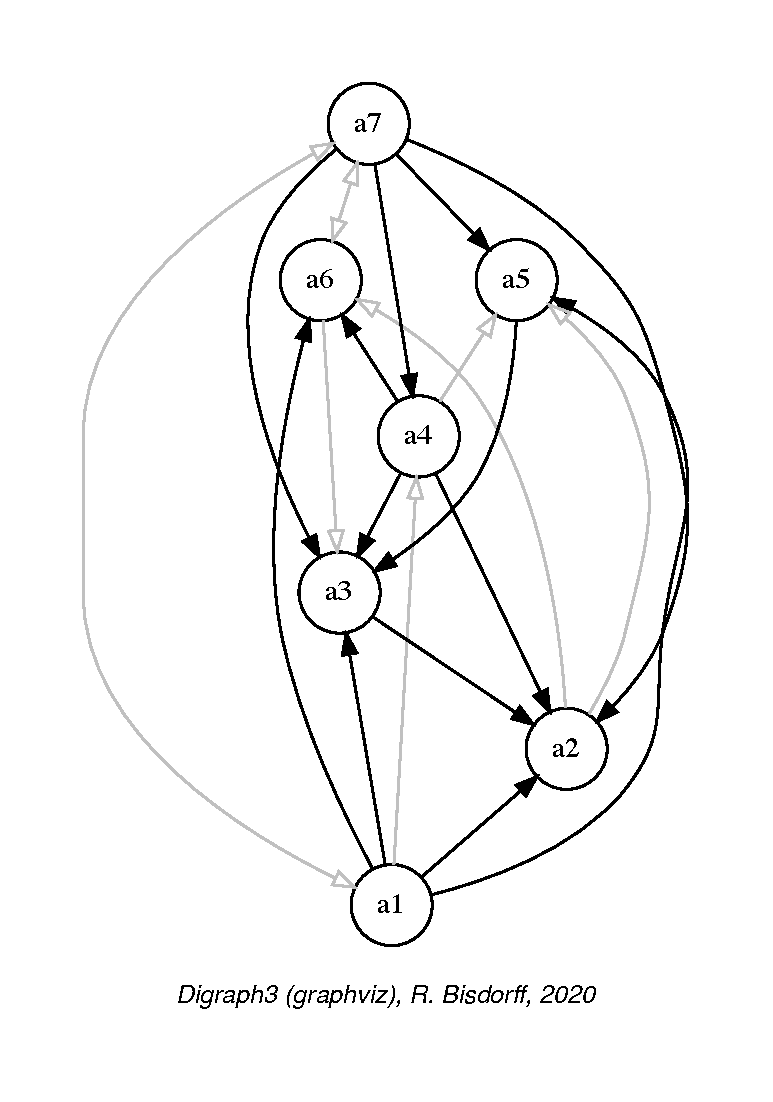
\includegraphics[width=5cm]{Figures/3-1-codualOdg.pdf}
\caption[The strict (codual) outranking digraph]{The strict (codual) outranking digraph. It becomes readily clear now from the picture that both alternatives \texttt{a1}  and \texttt{a7} are \emph{not outranked} by any other alternatives. Hence, \texttt{a1}  and \texttt{a7} appear as \emph{weak} \Condorcet winners and may be recommended as potential \emph{best} decision alternatives in this illustrative preference modelling example}
\label{fig:3.1}       % Give a unique label
\end{figure}
 
Many more tools for exploiting bipolar-valued outranking digraphs are available in the \Digraph resources \citep{BIS-2021b}.
\vspace{1cm}

In the methodological Part II, we present and discuss multiple criteria evaluation models and decision algorithms, like building a best choice recommendation, determining the winner of an election, computing linear rankings or quantile ratings with multiple incommensurable criteria.

%%%%%%%%%%%%%%%%%%%%%%%%%%%%%%%%%%%%
\phantomsection
\addcontentsline{toc}{section}{Notes}
\section*{Notes}

The seminal work on outranking digraphs goes back to the seventies and eighties when Bernard Roy \index{Roy@\textsl{B. Roy}} joined the just starting University Paris-Dauphine and founded there the '\emph{Laboratoire d’Analyse et de Modélisation de Systèmes pour l’Aide à la Décision}' (LAMSADE). The LAMSADE became the major site in the development of the outranking approach to multiple criteria decision aid. \citep*{ROY-1993}.

The ongoing success of the original \emph{outranking} concept stems from the fact that it is rooted in a sound pragmatism. The multiple criteria performance tableau, necessarily associated with a given outranking digraph, is indeed convincingly objective and meaningful \citep{ROY-1991}. And, ideas from social choice theory gave initially the insight that a pairwise voting mechanism à la \Condorcet could provide an order-statistical tool for aggregating a set of preference points of view into what M. Barbut\index{Barbut@\emph{M. Barbut}} called the \emph{central} \Condorcet point of view (\citealp{CON-1784} and \citealp{BAR-1980}); in fact the median of the multiple preference points of view, at minimal absolute \Kendall's\index{Kendall@\emph{M.G. Kendall}} ordinal correlation distance from all individual points of view (see Chap.~\ref{sec:16}).

Considering thus each performance criterion as a subset of unanimous voters and balancing the votes in favour against considerable counter-performances in disfavour gave eventually rise to the concept of \emph{outranking situation}, a distinctive feature of the Multiple Criteria Decision Aid approach \citep{BIS-2015}.  A modern definition would be : An alternative $x$ is said to \emph{outrank} alternative $y$ when – a \emph{significant majority} of criteria confirm that alternative $x$ has to be considered as \emph{at least as well evaluated as} an alternative $y$ (the \emph{concordance} argument); and – no discordant criterion opens to significant doubt the validity of the previous confirmation by revealing a considerable counter-performance of alternative $x$ compared to $y$ (the \emph{discordance} argument).

If the concordance argument was always well received, the discordance argument however, very confused in the beginning \citep{ROY-1966}, could only be handled in an epistemically correct and logically sound way by using a bipolar-valued epistemic logic (see Def.~\vref{def:3.1} and \citealp{BIS-2013}). The outranking situation had consequently to receive an explicit negative definition: An alternative $x$ is said to \emph{do not outrank} an alternative $y$ when – a \emph{significant majority} of criteria confirm that alternative $x$ has to be considered as \emph{not at least as well evaluated as} alternative $y$; and – no discordant criterion opens to significant doubt the validity of the previous confirmation by revealing a considerable \emph{better} performance of alternative $x$ compared to $y$.

Furthermore, the initial conjunctive aggregation of the concordance and discordance arguments had to be replaced by a disjunctive epistemic fusion operation, polarising in a logically and epistemically sound way the concordance with the discordance argument. This way, bipolar-valued outranking  digraphs gain two very useful properties from a measure theoretical perspective. They are \emph{weakly complete}; incomparability situations are no longer attested by the absence of positive outranking relations, but instead by epistemic indeterminateness. And they verify the \emph{coduality principle}: the negation of the epistemic ``\emph{at least as well evaluated as}'' situation corresponds formally to the strict converse epistemic ``\emph{less well evaluated than}'' situation.


%%%%%%% The chapter bibliography
%\normallatexbib
\clearpage
%\phantomsection
%\addcontentsline{toc}{section}{Chapter Bibliography}
%\chapter{Working with outranking digraphs}
\label{sec:3}

\abstract*{ In this chapter, we introduce the main formal object of this book, namely the bipolar-valued outranking digraph. With a randomly generated multiple criteria performance tableau, we construct the corresponding bipolar-valued outranking relation from pairwise comparisons. The resulting bipolar-valued outranking characteristics may be recoded. Finally, the codual outranking digraph gives us the associated strict outranking relation.}

\begin{quotation}
``\emph{The rule for the combination of independent concurrent arguments takes a very simple form when expressed in terms of the intensity of belief ... It is this: Take the sum of all the feelings of belief which would be produced separately by all the arguments pro, subtract from that the similar sum for arguments con, and the remainder is the feeling of belief which ought to have the whole. This is a proceeding which men often resort to, under the name of balancing reasons.}'' -- C.S. Peirce, The probability of induction (1878)
\end{quotation}
\vspace{1cm}

\abstract{ In this chapter, we introduce the main formal object of this book, namely the bipolar-valued outranking digraph. With a randomly generated multiple criteria performance tableau, we construct the corresponding bipolar-valued outranking relation from pairwise comparisons. The resulting bipolar-valued outranking characteristics may be recoded. Finally, the codual outranking digraph gives us the associated strict outranking relation.}


\section{The hybrid outranking digraph model}
\label{sec:3.1}

In the \texttt{outrankingDigraphs} module\index{outrankingDigraphs@\texttt{outrankingDigraphs} module}, the \texttt{BipolarOutrankingDigraph}\index{BipolarOutrankingDigraph@\texttt{BipolarOutrankingDigraph} class} class provides our standard \emph{outranking digraph} constructor. Such an instance represents a \emph{hybrid} object of both the \texttt{PerformanceTableau} type \emph{and} the \texttt{Outran\-kingDigraph} type \citep{BIS-2021b}.

A given \texttt{BipolarOutrankingDigraph} object contains hence always at least the following attributes:
\begin{enumerate}[topsep=3pt,partopsep=0pt]
\item \texttt{actions}: an ordered dictionary describing the potential decision actions or alternatives with \texttt{name} and \texttt{comment} attributes,
\item \texttt{objectives}: a possibly empty ordered dictionary of decision objectives with \texttt{name} and \texttt{comment} attributes, describing the multiple preference dimensions involved in the decision problem, 
\item \texttt{criteria}: an ordered dictionary of performance criteria, i.e. \emph{preferentially independent} and \emph{non-redundant} decimal-valued evaluation functions used for assessng the performance of each potential decision action with respect to a decision objective,
\item \texttt{evaluation}: a double dictionary gathering performance evaluations for each decision alternative on each criterion function. 
\item \texttt{valuationdomain}: a dictionary with three entries: the minimum ($-1.0$, \emph{certainly outranked}), the median ($0.0$, \emph{indeterminate}) and the maximum characteristic value ($+1.0$, \emph{certainly outranking}),
\item \texttt{relation}: a double dictionary defined on the Cartesian product of the set of decision alternatives capturing the credibility of the pairwise \emph{outranking situation} computed on the basis of the performance differences observed between couples of decision alternatives on the given family of criteria functions.   
\end{enumerate}

Let us consider, for instance, a random bipolar-valued outranking digraph with seven decision actions denoted \texttt{a1}, \texttt{a2}, ..., \texttt{a7}. We need therefore, first, to generate in Listing~\vref{list:3.1} a corresponding random performance tableau.
\begin{lstlisting}[caption={Generating a random performance tableau.},label=list:3.1]
>>> from perfTabs import RandomPerformanceTableau
>>> pt = RandomPerformanceTableau(numberOfActions=7,\
...                               seed=100)   
>>> pt
   *------- PerformanceTableau instance description ------*
    Instance class     : RandomPerformanceTableau
    Seed               : 100
    Instance name      : randomperftab
    Actions            : 7
    Criteria           : 7
    NaN proportion (%) : 6.1
>>> pt.showActions()
  *----- show digraphs actions --------------*
   key:  a1
    name:       action 1
    comment:    RandomPerformanceTableau() generated.
   key:  a2
    name:       action 2
    comment:    RandomPerformanceTableau() generated.
     ...
     ...
   key:  a7
    name:       action 7
    comment:    RandomPerformanceTableau() generated.
\end{lstlisting}

In this example we consider a family of seven \emph{equisignificant} cardinal \emph{criteria functions} \texttt{g1}, \texttt{g2}, ..., \texttt{g7}, measuring the performance of each alternative on a rational scale from $0.0$ (worst) to $100.00$ (best). In order to capture the evaluation procedures' potential \emph{uncertainty} and \emph{imprecision}, each criterion function \texttt{g1} to \texttt{g7} admits three performance \emph{discrimination thresholds} of $2.5$, $5.0$ and $80.0$ pts for warranting respectively any \emph{indifference}, \emph{preference} or \emph{considerable performance difference} situation.
\begin{lstlisting}[caption={Inspecting the performance criteria.},label=list:3.2]
>>> pt.showCriteria()
  *----  criteria -----*
   g1 'RandomPerformanceTableau() instance'
     Scale = [0.0, 100.0]
     Weight = 1.0
     Threshold ind : 2.50 + 0.00x ; percentile: 4.76
     Threshold pref : 5.00 + 0.00x ; percentile: 9.52
     Threshold veto : 80.00 + 0.00x ; percentile: 95.24
   g2 'RandomPerformanceTableau() instance'
     Scale = [0.0, 100.0]
     Weight = 1.0
     Threshold ind : 2.50 + 0.00x ; percentile: 6.67
     Threshold pref : 5.00 + 0.00x ; percentile: 6.67
     Threshold veto : 80.00 + 0.00x ; percentile: 100.00
      ...
      ...
   g7 'RandomPerformanceTableau() instance'
     Scale = [0.0, 100.0]
     Weight = 1.0
     Threshold ind : 2.50 + 0.00x ; percentile: 0.00
     Threshold pref : 5.00 + 0.00x ; percentile: 4.76
     Threshold veto : 80.00 + 0.00x ; percentile: 100.00
\end{lstlisting}

On criteria function \texttt{g1} (see Lines 6-8 in List.~\vref{list:3.2}) we observe, for instance, about $5\%$ of \emph{indifference} situations, about $90\%$ of \emph{preference} situations and about $5\%$ of \emph{considerable} performance difference situations.

The individual \emph{performance evaluation} of all decision alternative on each criterion are gathered in a \emph{performance table}.\index{showPerformanceTableau@\texttt{showPerformanceTableau()}}
\begin{lstlisting}[caption={Inspecting the performance evaluations},label=list:3.3]
>>> pt.showPerformanceTableau()
    *----  performance tableau -----*
     criteria |  'a1'  'a2'  'a3'  'a4'  'a5'  'a6'  'a7'   
     ---------|------------------------------------------
      'g1'    |  15.2  44.5  57.9  58.0  24.2  29.1  96.6  
      'g2'    |  82.3  43.9   NA   35.8  29.1  34.8  62.2  
      'g3'    |  44.2  19.1  27.7  41.5  22.4  21.5  56.9  
      'g4'    |  46.4  16.2  21.5  51.2  77.0  39.4  32.1  
      'g5'    |  47.7  14.8  79.7  67.5   NA   90.7  80.2  
      'g6'    |  69.6  45.5  22.0  33.8  31.8   NA   48.8  
      'g7'    |  82.9  41.7  12.8  21.9  75.7  15.4   6.0  
\end{lstlisting}

It is noteworthy to mention the three \emph{missing data} (\texttt{NA}) cases: action \texttt{a3} is missing, for instance, an evaluation on criterion \texttt{g2} (see Line 6 in List.~\vref{list:3.3}).
    
\section{The bipolar-valued outranking digraph}
\label{sec:3.2}

Given the previous random performance tableau \texttt{pt}, the \texttt{BipolarOutranking\-Digraph}\index{BipolarOutrankingDigraph@\texttt{BipolarOutrankingDigraph}} class constructor computes the corresponding \emph{bipolar-valued outranking digraph}. 
\begin{lstlisting}[caption={Example of random bipolar-valued outranking digraph.},label=list:3.4]
>>> from outrankingDigraphs import \
...                       BipolarOutrankingDigraph
>>> odg = BipolarOutrankingDigraph(pt)
>>> odg
  *------- Object instance description ------*
   Instance class       : BipolarOutrankingDigraph
   Instance name        : rel_randomperftab
   Actions              : 7
   Criteria             : 7
   Size                 : 20
   Determinateness (%)  : 63.27
   Valuation domain     : [-1.00;1.00]
   Attributes           : [
        'name', 'actions', 
	'criteria', 'evaluation', 'NA',
	'valuationdomain', 'relation', 
	'order', 'gamma', 'notGamma', ...
	]
\end{lstlisting}

The resulting digraph contains 20 positive (valid) outranking relations. And, the mean majority criteria significance support of all the pairwise outranking situations is $63.3\%$ (see Lines 9-10 in List.~\vref{list:3.4}).

We may inspect the complete $[-1.0,+1.0]$-valued adjacency table with the \texttt{showRelationTable()} method().\index{showRelationTable@\texttt{showRelationTable()}}
\begin{lstlisting}[caption={Inspecting the valued adjacency table.},label=list:3.5]
>>> odg.showRelationTable()
  * ---- Relation Table -----
   r(x,y)|  'a1'   'a2'   'a3'   'a4'   'a5'   'a6'   'a7'   
   ------|-------------------------------------------------
    'a1' | +1.00  +0.71  +0.29  +0.29  +0.29  +0.29  +0.00  
    'a2' | -0.71  +1.00  -0.29  -0.14  +0.14  +0.29  -0.57  
    'a3' | -0.29  +0.29  +1.00  -0.29  -0.14  +0.00  -0.29  
    'a4' | +0.00  +0.14  +0.57  +1.00  +0.29  +0.57  -0.43  
    'a5' | -0.29  +0.00  +0.14  +0.00  +1.00  +0.29  -0.29  
    'a6' | -0.29  +0.00  +0.14  -0.29  +0.14  +1.00  +0.00  
    'a7' | +0.00  +0.71  +0.57  +0.43  +0.29  +0.00  +1.00  
   Valuation domain: [-1.0; 1.0]
\end{lstlisting}

The \texttt{BipolarOutrankingDigraph}\index{BipolarOutrankingDigraph@\texttt{BipolarOutrankingDigraph}} class constructor computes from the given performance tableau $pt$ the characteristic value $r(x \succsim y)$ of a \emph{pairwise outranking} relation $x\, \succsim \,y$ in a default \emph{valuation domain} $[-1.0,+1.0]$ with the {\em median\/} value $0.0$ acting as \emph{indeterminate} characteristic value\footnote{See Definition~\vref{def:3.1} \citep{BIS-2013}}. 

\begin{definition}[Semantics of the bipolar-valued characteristic function $r$]\label{def:3.1}

\noindent The semantics of $r(x \succsim y)$ are the following:
\begin{itemize}[nosep]
\item [a.] When $r(x \succsim y) > 0.0$, it is more {\em True\/} than {\em False\/} that $x$ \emph{outranks} $y$, i.e. alternative $x$ is ``\emph{at least as well evaluated as}'' alternative $y$ on a weighted majority of criteria {\bf and} there is no considerable negative performance difference observed in disfavour of $x$,
\item [b.] When $r(x \succsim y) < 0.0$, it is more {\em False\/} than {\em True\/} that $x$ \emph{outranks} $y$, i.e. alternative $x$ is {\bf not} ``\emph{at least as well evaluated as} alternative $y$ on a weighted majority of criteria than alternative $y$ {\bf and} there is no considerable positive performance difference observed in favour of $x$,
\item [c.] When $r(x \succsim y) = 0.0$, it is {\bf indeterminate} whether $x$ outranks $y$ or not.
\end{itemize}
\end{definition}

\section{Pairwise comparisons}
\label{sec:3.3}

From above given semantics, we notice in line 5 in Listing~\vref{list:3.5} that \texttt{a1} outranks \texttt{a2}: $r(a1 \succsim a2) + 0.71$), but not \texttt{a7}: $r(a1 \succsim a7) = 0.0$). In order to comprehend the characteristic values shown in the outranking relation table, we can inspect with the \texttt{showPairwiseComparison()} method\index{showPairwiseComparison@\texttt{showPairwiseComparison()}} the details of the pairwise multiple criteria comparison between, for instance, alternatives \texttt{a1} and \texttt{a2}.
\begin{lstlisting}[caption={Inspecting a pairwise multiple criteria comparison},label=list:3.6]
>>> odg.showPairwiseComparison('a1','a2')
  *------------  pairwise comparison ----*
   Comparing actions : (a1, a2)
   crit. wght. g(a1)  g(a2)   diff  | ind   pref    r() 
   -------------------------------  	 --------------------
    g1   1.00  15.17  44.51  -29.34 | 2.50  5.00   -1.00 
    g2   1.00  82.29  43.90  +38.39 | 2.50  5.00   +1.00 
    g3   1.00  44.23  19.10  +25.13 | 2.50  5.00   +1.00 
    g4   1.00  46.37  16.22  +30.15 | 2.50  5.00   +1.00 
    g5   1.00  47.67  14.81  +32.86 | 2.50  5.00   +1.00 
    g6   1.00  69.62  45.49  +24.13 | 2.50  5.00   +1.00 
    g7   1.00  82.88  41.66  +41.22 | 2.50  5.00   +1.00 
    Valuation in range: -7.00 to +7.00;          -------
       r(a1,a2): +5.00/7.00 = +0.71                +5.00
\end{lstlisting}

The outranking characteristic value $r(a1 \succsim a2)$ represents the relative \emph{majority margin} resulting from the difference between the significance weights of the criteria in favour and the significance weights of the criteria in disfavour of the statement that alternative \texttt{a1} is ``\emph{at least as well evaluated as}'' alternative \texttt{a2}. No considerable performance difference being observed, no polarising situation is triggered in this pairwise comparison.

Such a polarised situation is however observed when we compare the evaluations of alternatives \texttt{a1} and \texttt{a7} with the \texttt{showPairwiseOutrankings()} method. \index{showPairwiseoutrankings@\texttt{showPairwiseOutrankings()}}
\begin{lstlisting}[caption={Pairwise comparison with considerable performance difference},label=list:3.7,basicstyle=\ttfamily\scriptsize]
>>> odg.showPairwiseoutrankings('a1','a7')
  *------------  pairwise comparison ----*
   Comparing actions : (a1, a7)
   crit. wght. g(a1)  g(a7)   diff  | ind   pref    r()  |  v     veto
   -------------------------------   ------------------   -----------
    g1   1.00  15.17  96.58  -81.41 | 2.50  5.00   -1.00 | 80.00 -1.00
    g2   1.00  82.29  62.22  +20.07 | 2.50  5.00   +1.00 | 
    g3   1.00  44.23  56.90  -12.67 | 2.50  5.00   -1.00 | 
    g4   1.00  46.37  32.06  +14.31 | 2.50  5.00   +1.00 | 
    g5   1.00  47.67  80.16  -32.49 | 2.50  5.00   -1.00 | 
    g6   1.00  69.62  48.80  +20.82 | 2.50  5.00   +1.00 | 
    g7   1.00  82.88   6.05  +76.83 | 2.50  5.00   +1.00 | 
   ----------------------------------------
   Valuation in range: -7.00 to +7.00; r(x,y)= +1/7 => 0.0
  *------------  pairwise comparison ----*
   Comparing actions : (a1, a7)
   crit. wght. g(a7)  g(a1)   diff  | ind   pref    r()  |  v     veto
   -------------------------------   ------------------   -----------
    g1   1.00  96.58  15.17  +81.41 | 2.50  5.00   +1.00 | 80.00 +1.00
    g2   1.00  62.22  82.29  -20.07 | 2.50  5.00   -1.00 | 
    g3   1.00  56.90  44.23  +12.67 | 2.50  5.00   +1.00 | 
    g4   1.00  32.06  46.37  -14.31 | 2.50  5.00   -1.00 | 
    g5   1.00  80.16  47.67  +32.49 | 2.50  5.00   +1.00 | 
    g6   1.00  48.80  69.62  -20.82 | 2.50  5.00   -1.00 | 
    g7   1.00   6.05  82.88  -76.83 | 2.50  5.00   -1.00 | 
   ----------------------------------------
   Valuation in range: -7.00 to +7.00; r(x,y)= -1/7 => 0.0
\end{lstlisting}

This time, we observe a $(1/7 + 1)/2 = 57.1\%$ majority of criteria significance warranting a ``\emph{at least as well evaluated as}'' situation between alternative \texttt{a1} and alternative \texttt{a7}. Yet, we also observe a considerable \emph{negative} performance difference on criterion \texttt{g1} (see Line 6 in List.~\vref{list:3.7}). Both contradictory facts trigger eventually in Line 14 an \emph{indeterminate} outranking situation. The inverse polarisation effect appears when considering in Lines 19-25 the converse performance differences between alternative \texttt{a7} and alternative \texttt{a1}. The considerable better performing situation on criterion \texttt{g1} makes doubtful the otherwise ``\emph{not at least as well evaluated as}'' situation (see Lines 19 and 27).

Notice that the occurrence in a pairwise comparison of conjointly considerable positive and negative performance differences will also trigger an indeterminate outranking situation. When observing at the same time a positive (resp. negative) ``\emph{at least as well evaluated as}'' situation and one or more considerable positive (resp. negative) performance difference, the outranking situation gets validated (resp. invalidated) for certain \citep{BIS-2013}.

\section{Recoding the characteristic valuation domain}
\label{sec:3.4}

All outranking digraphs, being of root \texttt{Digraph} type, inherit the methods available under this latter class. The characteristic valuation domain of a digraph can, for instance, be recoded with the \texttt{recodeValuation()}\index{recodeValuation@\emph{recodeValuation()}} method to the \emph{integer} range $[-7,+7]$, i.e. plus or minus the total significance weights of the family of criteria considered in this example instance \texttt{odg}.
\begin{lstlisting}[caption={Recoding the digraph valuation},label=list:3.8]
>>> odg.recodeValuation(-7,+7)
>>> odg.valuationdomain['hasIntegerValuation'] = True
>>> Digraph.showRelationTable(odg,ReflexiveTerms=False)
  * ---- Relation Table -----
   r(x,y)  |  'a1'  'a2'  'a3'  'a4'  'a5'  'a6'  'a7'	  
  ---------|------------------------------------------
    'a1'   |    -    +5    +2    +2    +2    +2     0	 
    'a2'   |   -5     -    -1    -1    +1    +2    -4	 
    'a3'   |   -1    +2     -    -1    -1     0    -1	 
    'a4'   |    0    +1    +4     -    +2    +4    -3	 
    'a5'   |   -1     0    +1     0     -    +2    -1	 
    'a6'   |   -1     0    +1    -1    +1     -     0	 
    'a7'   |    0    +5    +4    +3    +2     0     -	 
    Valuation domain: [-7;+7]
\end{lstlisting}

Notice in Listing~\vref{list:3.8} that the self comparison characteristics $r(x \succsim x)$ may be ignored by setting the \texttt{ReflexiveTerms} Boolean parameter to \texttt{False}. Mind that the trivial reflexive terms of outranking relations are ignored in some of the \Digraph methods. 

\section{The strict outranking digraph}
\label{sec:3.5}

From theory we know that a bipolar-valued outranking digraph is \emph{weakly complete}, i.e. if $r(x \succsim y) < 0.0$ then $r(y \succsim x) \geq 0.0$. From this property follows that a bipolar-valued outranking digraph verifies the \emph{coduality principle}\index{coduality principle}: the \emph{dual}\footnote{Not to be confused with the dual graph of a plane graph $g$ that has a vertex for each face of $g$. Here we mean the \emph{less than} (strict converse) relation corresponding to a \emph{greater or equal} relation, or the \emph{less than or equal} relation corresponding to a (strict) \emph{better than} relation.} --strict negation-- of the \emph{converse} --inverse-- of the outranking relation $(x \succsim y)$ corresponds to its asymmetric \emph{strict outranking} part $(x \succnsim y)$  \citep{BIS-2013, ADT-L7}.

We may visualize the \emph{codual} (\emph{strict}) outranking digraph with a graphviz drawing \footnote{The \texttt{exportGraphViz()} method is depending on drawing tools from the graphviz software (https://graphviz.org/). On Linux Ubuntu or Debian you may try \texttt{sudo apt-get install graphviz} to install them. There are ready \emph{dmg} installers for Mac OSX.}.\index{graphviz}
\begin{lstlisting}
>>> cdodg = -(~odg)
>>> cdodg.exportGraphViz('codualOdg')
  *---- exporting a dot file for GraphViz tools ---------*
   Exporting to codualOdg.dot
   dot -Grankdir=BT -Tpng codualOdg.dot -o codualOdg.png
\end{lstlisting}
\begin{figure}[ht]
\sidecaption[t]
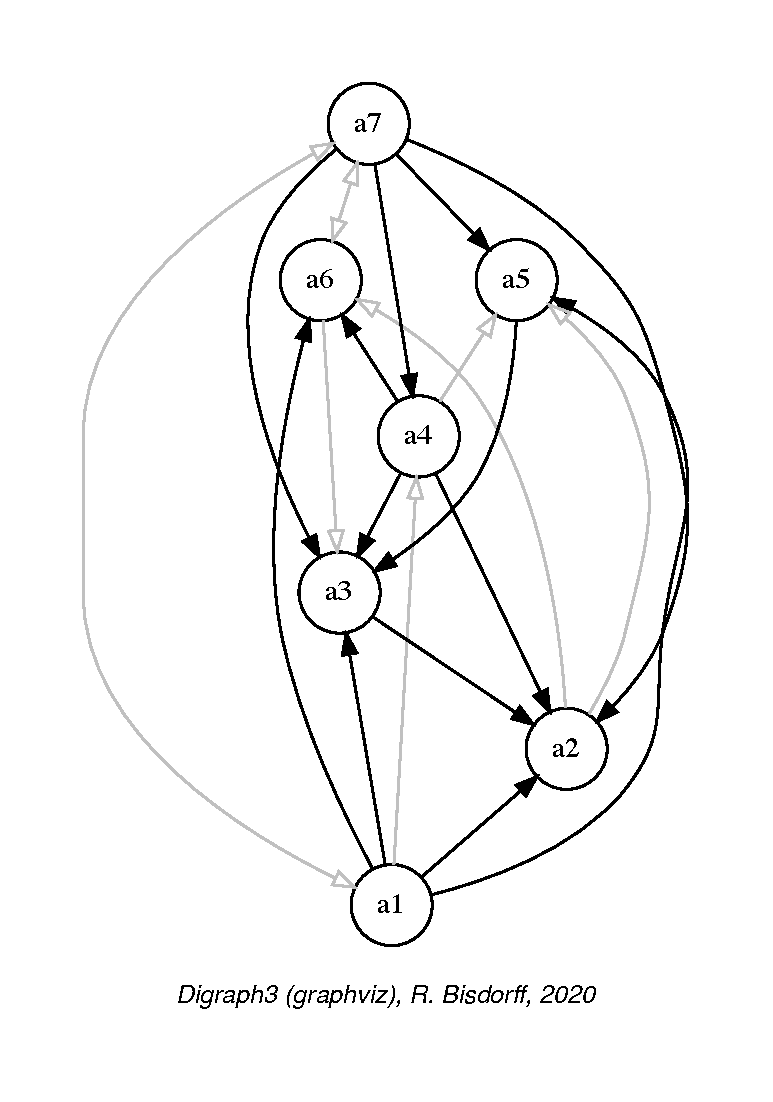
\includegraphics[width=5cm]{Figures/3-1-codualOdg.pdf}
\caption[The strict (codual) outranking digraph]{The strict (codual) outranking digraph. It becomes readily clear now from the picture that both alternatives \texttt{a1}  and \texttt{a7} are \emph{not outranked} by any other alternatives. Hence, \texttt{a1}  and \texttt{a7} appear as \emph{weak} \Condorcet winners and may be recommended as potential \emph{best} decision alternatives in this illustrative preference modelling example}
\label{fig:3.1}       % Give a unique label
\end{figure}
 
Many more tools for exploiting bipolar-valued outranking digraphs are available in the \Digraph resources \citep{BIS-2021b}.
\vspace{1cm}

In the methodological Part II, we present and discuss multiple criteria evaluation models and decision algorithms, like building a best choice recommendation, determining the winner of an election, computing linear rankings or quantile ratings with multiple incommensurable criteria.

%%%%%%%%%%%%%%%%%%%%%%%%%%%%%%%%%%%%
\phantomsection
\addcontentsline{toc}{section}{Notes}
\section*{Notes}

The seminal work on outranking digraphs goes back to the seventies and eighties when Bernard Roy \index{Roy@\textsl{B. Roy}} joined the just starting University Paris-Dauphine and founded there the '\emph{Laboratoire d’Analyse et de Modélisation de Systèmes pour l’Aide à la Décision}' (LAMSADE). The LAMSADE became the major site in the development of the outranking approach to multiple criteria decision aid. \citep*{ROY-1993}.

The ongoing success of the original \emph{outranking} concept stems from the fact that it is rooted in a sound pragmatism. The multiple criteria performance tableau, necessarily associated with a given outranking digraph, is indeed convincingly objective and meaningful \citep{ROY-1991}. And, ideas from social choice theory gave initially the insight that a pairwise voting mechanism à la \Condorcet could provide an order-statistical tool for aggregating a set of preference points of view into what M. Barbut\index{Barbut@\emph{M. Barbut}} called the \emph{central} \Condorcet point of view (\citealp{CON-1784} and \citealp{BAR-1980}); in fact the median of the multiple preference points of view, at minimal absolute \Kendall's\index{Kendall@\emph{M.G. Kendall}} ordinal correlation distance from all individual points of view (see Chap.~\ref{sec:16}).

Considering thus each performance criterion as a subset of unanimous voters and balancing the votes in favour against considerable counter-performances in disfavour gave eventually rise to the concept of \emph{outranking situation}, a distinctive feature of the Multiple Criteria Decision Aid approach \citep{BIS-2015}.  A modern definition would be : An alternative $x$ is said to \emph{outrank} alternative $y$ when – a \emph{significant majority} of criteria confirm that alternative $x$ has to be considered as \emph{at least as well evaluated as} an alternative $y$ (the \emph{concordance} argument); and – no discordant criterion opens to significant doubt the validity of the previous confirmation by revealing a considerable counter-performance of alternative $x$ compared to $y$ (the \emph{discordance} argument).

If the concordance argument was always well received, the discordance argument however, very confused in the beginning \citep{ROY-1966}, could only be handled in an epistemically correct and logically sound way by using a bipolar-valued epistemic logic (see Def.~\vref{def:3.1} and \citealp{BIS-2013}). The outranking situation had consequently to receive an explicit negative definition: An alternative $x$ is said to \emph{do not outrank} an alternative $y$ when – a \emph{significant majority} of criteria confirm that alternative $x$ has to be considered as \emph{not at least as well evaluated as} alternative $y$; and – no discordant criterion opens to significant doubt the validity of the previous confirmation by revealing a considerable \emph{better} performance of alternative $x$ compared to $y$.

Furthermore, the initial conjunctive aggregation of the concordance and discordance arguments had to be replaced by a disjunctive epistemic fusion operation, polarising in a logically and epistemically sound way the concordance with the discordance argument. This way, bipolar-valued outranking  digraphs gain two very useful properties from a measure theoretical perspective. They are \emph{weakly complete}; incomparability situations are no longer attested by the absence of positive outranking relations, but instead by epistemic indeterminateness. And they verify the \emph{coduality principle}: the negation of the epistemic ``\emph{at least as well evaluated as}'' situation corresponds formally to the strict converse epistemic ``\emph{less well evaluated than}'' situation.


%%%%%%% The chapter bibliography
%\normallatexbib
\clearpage
%\phantomsection
%\addcontentsline{toc}{section}{Chapter Bibliography}
%\input{02-mainMatters/03-chapterOutrankingDigraphs.bbl}
\bibliographystyle{spbasic}
\bibliography{03-backMatters/reference}

\bibliographystyle{spbasic}
\bibliography{03-backMatters/reference}

\bibliographystyle{spbasic}
\bibliography{03-backMatters/reference}
